% Options for packages loaded elsewhere
\PassOptionsToPackage{unicode}{hyperref}
\PassOptionsToPackage{hyphens}{url}
%
\documentclass[
  oneside]{book}
\usepackage{amsmath,amssymb}
\usepackage{lmodern}
\usepackage{ifxetex,ifluatex}
\ifnum 0\ifxetex 1\fi\ifluatex 1\fi=0 % if pdftex
  \usepackage[T1]{fontenc}
  \usepackage[utf8]{inputenc}
  \usepackage{textcomp} % provide euro and other symbols
\else % if luatex or xetex
  \usepackage{unicode-math}
  \defaultfontfeatures{Scale=MatchLowercase}
  \defaultfontfeatures[\rmfamily]{Ligatures=TeX,Scale=1}
\fi
% Use upquote if available, for straight quotes in verbatim environments
\IfFileExists{upquote.sty}{\usepackage{upquote}}{}
\IfFileExists{microtype.sty}{% use microtype if available
  \usepackage[]{microtype}
  \UseMicrotypeSet[protrusion]{basicmath} % disable protrusion for tt fonts
}{}
\makeatletter
\@ifundefined{KOMAClassName}{% if non-KOMA class
  \IfFileExists{parskip.sty}{%
    \usepackage{parskip}
  }{% else
    \setlength{\parindent}{0pt}
    \setlength{\parskip}{6pt plus 2pt minus 1pt}}
}{% if KOMA class
  \KOMAoptions{parskip=half}}
\makeatother
\usepackage{xcolor}
\IfFileExists{xurl.sty}{\usepackage{xurl}}{} % add URL line breaks if available
\IfFileExists{bookmark.sty}{\usepackage{bookmark}}{\usepackage{hyperref}}
\hypersetup{
  pdftitle={Economic Time Series Modeling and Forecasting},
  pdfauthor={David Ubilava},
  hidelinks,
  pdfcreator={LaTeX via pandoc}}
\urlstyle{same} % disable monospaced font for URLs
\usepackage{color}
\usepackage{fancyvrb}
\newcommand{\VerbBar}{|}
\newcommand{\VERB}{\Verb[commandchars=\\\{\}]}
\DefineVerbatimEnvironment{Highlighting}{Verbatim}{commandchars=\\\{\}}
% Add ',fontsize=\small' for more characters per line
\usepackage{framed}
\definecolor{shadecolor}{RGB}{248,248,248}
\newenvironment{Shaded}{\begin{snugshade}}{\end{snugshade}}
\newcommand{\AlertTok}[1]{\textcolor[rgb]{0.94,0.16,0.16}{#1}}
\newcommand{\AnnotationTok}[1]{\textcolor[rgb]{0.56,0.35,0.01}{\textbf{\textit{#1}}}}
\newcommand{\AttributeTok}[1]{\textcolor[rgb]{0.77,0.63,0.00}{#1}}
\newcommand{\BaseNTok}[1]{\textcolor[rgb]{0.00,0.00,0.81}{#1}}
\newcommand{\BuiltInTok}[1]{#1}
\newcommand{\CharTok}[1]{\textcolor[rgb]{0.31,0.60,0.02}{#1}}
\newcommand{\CommentTok}[1]{\textcolor[rgb]{0.56,0.35,0.01}{\textit{#1}}}
\newcommand{\CommentVarTok}[1]{\textcolor[rgb]{0.56,0.35,0.01}{\textbf{\textit{#1}}}}
\newcommand{\ConstantTok}[1]{\textcolor[rgb]{0.00,0.00,0.00}{#1}}
\newcommand{\ControlFlowTok}[1]{\textcolor[rgb]{0.13,0.29,0.53}{\textbf{#1}}}
\newcommand{\DataTypeTok}[1]{\textcolor[rgb]{0.13,0.29,0.53}{#1}}
\newcommand{\DecValTok}[1]{\textcolor[rgb]{0.00,0.00,0.81}{#1}}
\newcommand{\DocumentationTok}[1]{\textcolor[rgb]{0.56,0.35,0.01}{\textbf{\textit{#1}}}}
\newcommand{\ErrorTok}[1]{\textcolor[rgb]{0.64,0.00,0.00}{\textbf{#1}}}
\newcommand{\ExtensionTok}[1]{#1}
\newcommand{\FloatTok}[1]{\textcolor[rgb]{0.00,0.00,0.81}{#1}}
\newcommand{\FunctionTok}[1]{\textcolor[rgb]{0.00,0.00,0.00}{#1}}
\newcommand{\ImportTok}[1]{#1}
\newcommand{\InformationTok}[1]{\textcolor[rgb]{0.56,0.35,0.01}{\textbf{\textit{#1}}}}
\newcommand{\KeywordTok}[1]{\textcolor[rgb]{0.13,0.29,0.53}{\textbf{#1}}}
\newcommand{\NormalTok}[1]{#1}
\newcommand{\OperatorTok}[1]{\textcolor[rgb]{0.81,0.36,0.00}{\textbf{#1}}}
\newcommand{\OtherTok}[1]{\textcolor[rgb]{0.56,0.35,0.01}{#1}}
\newcommand{\PreprocessorTok}[1]{\textcolor[rgb]{0.56,0.35,0.01}{\textit{#1}}}
\newcommand{\RegionMarkerTok}[1]{#1}
\newcommand{\SpecialCharTok}[1]{\textcolor[rgb]{0.00,0.00,0.00}{#1}}
\newcommand{\SpecialStringTok}[1]{\textcolor[rgb]{0.31,0.60,0.02}{#1}}
\newcommand{\StringTok}[1]{\textcolor[rgb]{0.31,0.60,0.02}{#1}}
\newcommand{\VariableTok}[1]{\textcolor[rgb]{0.00,0.00,0.00}{#1}}
\newcommand{\VerbatimStringTok}[1]{\textcolor[rgb]{0.31,0.60,0.02}{#1}}
\newcommand{\WarningTok}[1]{\textcolor[rgb]{0.56,0.35,0.01}{\textbf{\textit{#1}}}}
\usepackage{longtable,booktabs,array}
\usepackage{calc} % for calculating minipage widths
% Correct order of tables after \paragraph or \subparagraph
\usepackage{etoolbox}
\makeatletter
\patchcmd\longtable{\par}{\if@noskipsec\mbox{}\fi\par}{}{}
\makeatother
% Allow footnotes in longtable head/foot
\IfFileExists{footnotehyper.sty}{\usepackage{footnotehyper}}{\usepackage{footnote}}
\makesavenoteenv{longtable}
\usepackage{graphicx}
\makeatletter
\def\maxwidth{\ifdim\Gin@nat@width>\linewidth\linewidth\else\Gin@nat@width\fi}
\def\maxheight{\ifdim\Gin@nat@height>\textheight\textheight\else\Gin@nat@height\fi}
\makeatother
% Scale images if necessary, so that they will not overflow the page
% margins by default, and it is still possible to overwrite the defaults
% using explicit options in \includegraphics[width, height, ...]{}
\setkeys{Gin}{width=\maxwidth,height=\maxheight,keepaspectratio}
% Set default figure placement to htbp
\makeatletter
\def\fps@figure{htbp}
\makeatother
\setlength{\emergencystretch}{3em} % prevent overfull lines
\providecommand{\tightlist}{%
  \setlength{\itemsep}{0pt}\setlength{\parskip}{0pt}}
\setcounter{secnumdepth}{5}
\ifluatex
  \usepackage{selnolig}  % disable illegal ligatures
\fi

\title{Economic Time Series Modeling and Forecasting}
\author{David Ubilava}
\date{August 2021}

\begin{document}
\maketitle

{
\setcounter{tocdepth}{1}
\tableofcontents
}
\hypertarget{preamble}{%
\chapter*{Preamble}\label{preamble}}
\addcontentsline{toc}{chapter}{Preamble}

These notes are prepared to teach an undergraduate-level course on economic forecasting. The content is presented in four parts. The first part, \emph{Preliminaries}, introduces the concept of forecasting in time series context. The second part, \emph{Deterministic Time Series Models}, covers trends and seasonal models. The third part, \emph{Dynamic Time Series Models}, covers linear, multivariate, and nonlinear autoregressive processes. The fourth part, \emph{Forecast Assessment}, goes over forecast evaluation and combination routines, and forecast accuracy tests.

\hypertarget{preliminaries}{%
\chapter*{Preliminaries}\label{preliminaries}}
\addcontentsline{toc}{chapter}{Preliminaries}

\hypertarget{introduction-to-forecasting}{%
\chapter{Introduction to Forecasting}\label{introduction-to-forecasting}}

Economic events tend to co-occur, precede, or succeed one another. Understanding the essence of such relationships -- that is, identifying causal mechanisms that facilitate correlation among economic variables -- is at the core of econometric analysis. Throughout a relatively brief history of the study of econometrics, numerous methods and techniques have been proposed and developed -- all aimed to give an empirical content to economic models. These methods and techniques allow us to test theories, evaluate policy outcomes, etc.

Econometric models rely on correct (and accurate) identification of the causal mechanism in the underlying process. But they are also predictive by nature -- they help us make economic forecasts even when the causal mechanism may not be well identified. In other words, while correlation does not necessarily imply causality, if the goal is to make a forecast, a mere correlation might as well suffice.

Roots of forecasting extend very much to the beginning of human history. In their desire to predict the future, people have attempted to make forecasts of their own, or have used services of others. Fortunetellers, for example, have been forecast experts of some sort, basing their predictions on magic. They are less common in the current age. Astrologers, who rely on astronomical phenomena to foresee the future, maintain their relevance to this date. Over time, and particularly with the development of the study of econometrics, more rigorous forecasting methods have been introduced and developed. All methods -- primitive or complex, spurious or scientifically substantiated -- have one thing in common: they all rely (or, at least, pretend to rely) on \emph{information}.

Information is key in forecasting. It comes in many forms, but after it is organized and stored, what we end up with is data. A diverse set of forecasting methods typically rely on insights from econometric analysis of time series -- chronologically stored data, collected at regular intervals over a period of time. In time series analysis, the implied assumption is that the past tends to repeat itself, at least to some extent. So, if we well study the past, we \emph{may} be able to forecast an event with some degree of accuracy.

Accurate forecasting is difficult. No matter how rich the available data are, or how well the econometric model fits the data, there still is a surprise element concerning the forecast -- something that has never happened in past, and is only specific to the future. And because of this, there is no such thing as precise forecast, even if by fluke we were to exactly predict an outcome of an event. But some forecasts are better than others. And in search of such forecasts the study of time series econometrics has evolved.

\hypertarget{stochastic-process-and-time-series}{%
\chapter{Stochastic Process and Time Series}\label{stochastic-process-and-time-series}}

Time series are realizations of a chronologically stored sequence of random variables. This sequence of random variables is referred to as the \emph{stochastic process}. Thus, a time series is a realisation of the stochastic process. We index time periods as \(1,2,\ldots,T\), and denote the set of observations as \(\{y_1,\ldots,y_T\}\). One can view a time series as a finite sample from an underlying doubly--infinite sequence: \(\{\ldots,y_{-1},y_{0},y_1,y_2,\ldots,y_T,y_{T+1},y_{T+2},\ldots\}\).

\hypertarget{stationarity}{%
\section{Stationarity}\label{stationarity}}

If all random variables, from where the time series are drawn, have the same distribution, then we refert to such time series as \emph{stationary}. Stationarity is an important feature, and the assumption, on which the time series analysis heavily relies.

Before diving any further into the concepts and methods of time series econometrics, consider the simplest kind of time series comprised of realizations from independent and identically distributed random variable with zero mean and constant variance: \(\varepsilon_t \sim iid\left(0,\sigma^2\right)\). The following graph plots this time series against time.

\begin{figure}
\centering
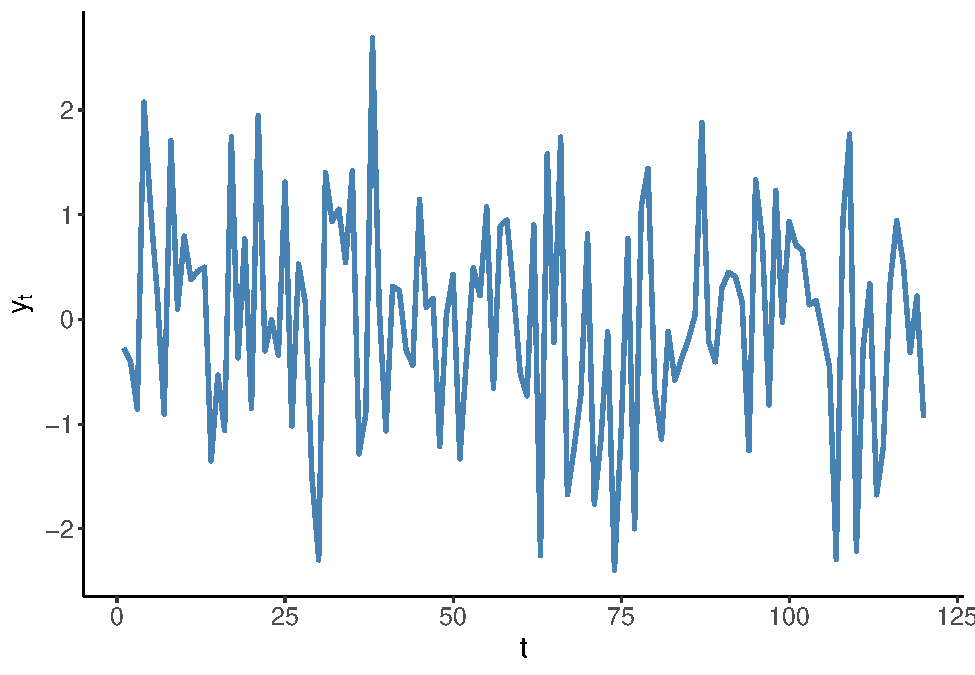
\includegraphics{forecasting_files/figure-latex/white-noise-1.pdf}
\caption{\label{fig:white-noise}White noise: an illustration}
\end{figure}

Such time series are referred to as \emph{white noise}. That is, a time series, \(y\), is a white noise process if:
\begin{align*}
& E(y_t) = 0,\;~\forall~t\\
& Var(y_t) = \sigma^2,\;~\forall~t\\
& Cov(y_t,y_{t-k}) = 0,\;~\forall~k \ne 0
\end{align*}

Because each observation is drawn from the same distribution, white noise is a stationary time series. Indeed, it is a special type of stationary time series insofar as its mean, variance, and covariance are time-invariant. Note, for a time series to be stationary, the mean doesn't need to be zero (as long as it is constant over time), nor covariances need to be equal to zero (as long as they are constant over time, though they may vary with \(k\)). Thus, \(\{y_t\}\) is stationary if the mean and variance are independent of \(t\), and the autocovariances are independent of \(t\) for all \(k\).

\hypertarget{serial-dependence}{%
\section{Serial Dependence}\label{serial-dependence}}

In fact, it is more of a norm rather than an exception for a time series to be correlated over time. Indeed, because of the sequential nature of time series, we commonly observe dependence among the temporally adjacent time series. That is, for most economic time series, we would expect \(y_t\) and \(y_{t-1}\) to be correlated. Such correlations are referred to as \emph{autocorrelations}, and are given by: \[\rho_k=Cor(y_t,y_{t-k}) = \frac{Cov(y_t,y_{t-k})}{Var(y_t)},\;~~k=1,2,\ldots\]

Autocorrelations are commonly illustrated via the so-called \emph{autocorrelogram}, which plots the sequence of autocorrelation coefficients against the lags at which these coefficients are obtained. For example, an autocorrelogram of the previously illustrated white noise process is as follows:

\begin{figure}
\centering
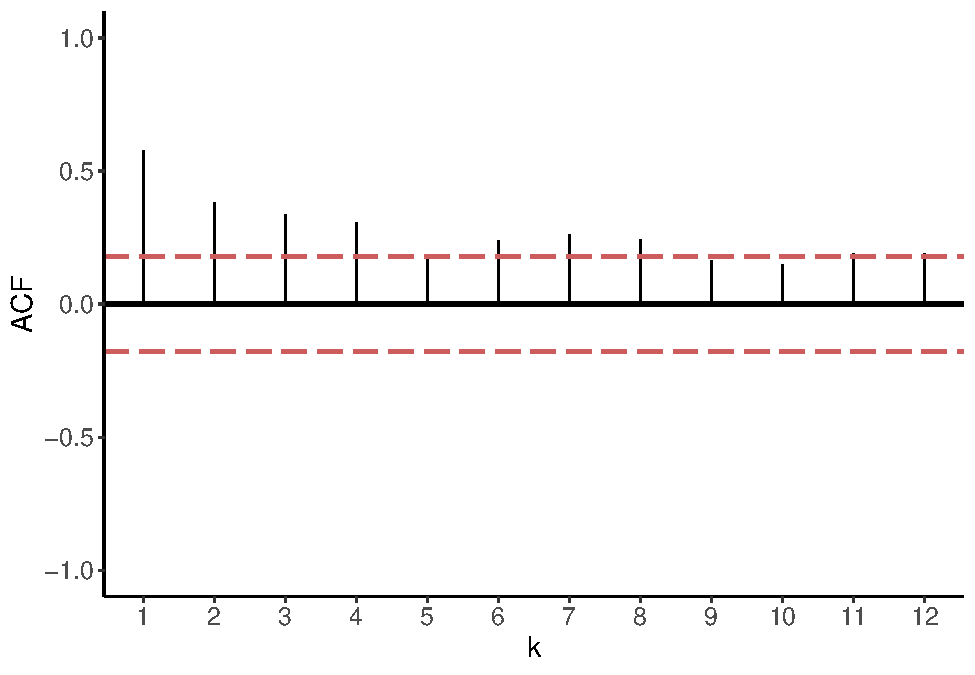
\includegraphics{forecasting_files/figure-latex/acf-1.pdf}
\caption{\label{fig:acf}Autocorrelation}
\end{figure}

For each \(k\), the vertical line extending from zero represents the autocorrelation coefficient at that lag. The red dashed lines denote the 90\% confidence interval, given by \(\pm 1.96/\sqrt{T}\), where \(T\) is the length of the time series.

Another relevant measure for time series dependence is partial autocorrelation, which is correlation between \(y_t\) and \(y_{t-k}\) net of any correlations between \(y_t\) and \(y_{t-k+j}\), for all \(j=1,\ldots,k-1\). Similar to autocorrelations, partial autocorrelations can also be illustrated using autocorrelograms:

\begin{figure}
\centering
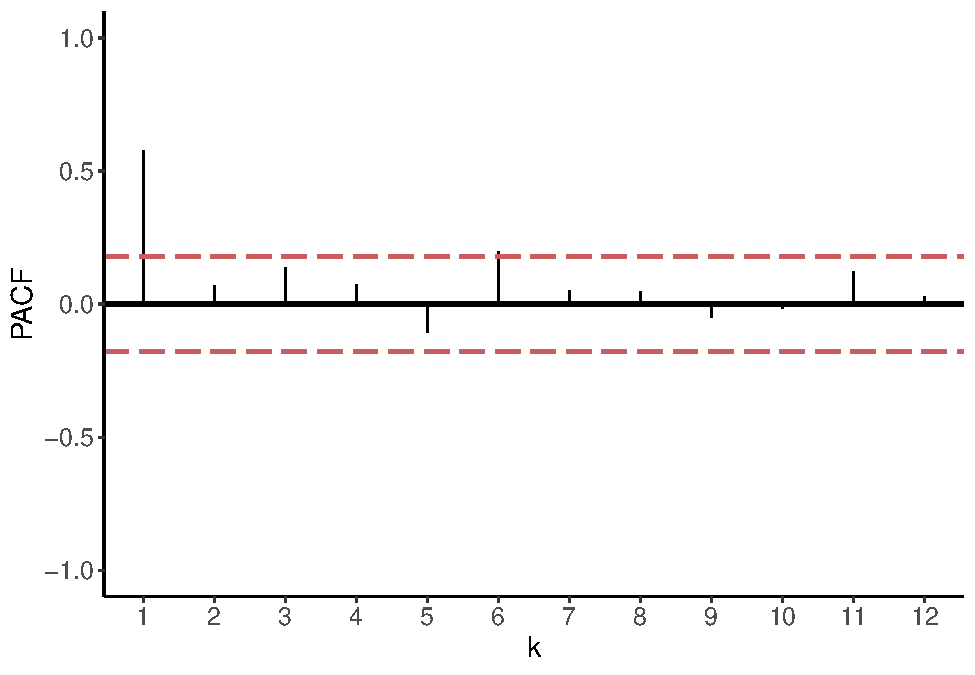
\includegraphics{forecasting_files/figure-latex/pacf-1.pdf}
\caption{\label{fig:pacf}Partial Autocorrelation}
\end{figure}

\hypertarget{transformations}{%
\section{Transformations}\label{transformations}}

It is common to transform time series by taking logarithms, differences, or differences of logarithms (growth rates). Such transformations usually are done to work with the suitable variable for the desired econometric analysis. For example, if an economic time series is characterized by an apparent exponential growth (e.g., real GDP), by taking natural logarithms the time series ``flatten'\,' and the fluctuations become proportionate. The difference operator is denoted by \(\Delta\), so that \(\Delta y_t = y_t-y_{t-1}\). The following three graphs illustrate (i) a time series with an apparent exponential growth, (ii) the natural logarithm of this time series, and (iii) their differences (i.e., the log-differences of the original series).

\begin{figure}
\centering
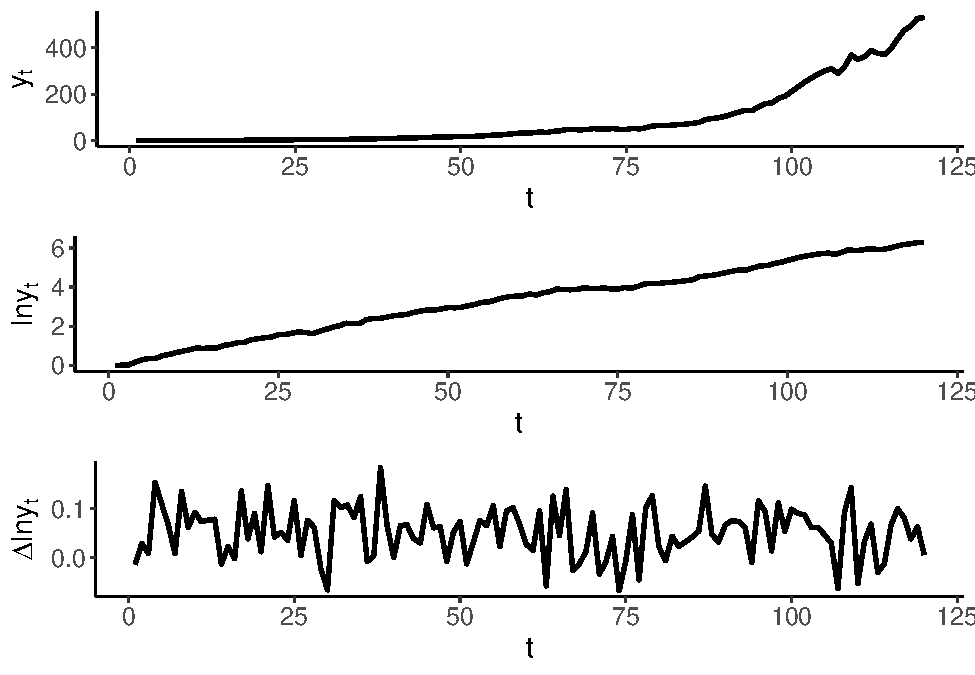
\includegraphics{forecasting_files/figure-latex/ts-1.pdf}
\caption{\label{fig:ts}A time series and its transformations}
\end{figure}

\hypertarget{basics-of-forecasting}{%
\chapter{Basics of Forecasting}\label{basics-of-forecasting}}

\hypertarget{optimal-forecast}{%
\section{Optimal Forecast}\label{optimal-forecast}}

A forecast is a random variable which has some distribution and, thus, moments. The simplest form of a forecast is a point forecast (usually a mean of the distribution, but can be a median or, indeed, any quantile).

A point forecast made in period \(t\) for horizon \(h\) can be denoted as \(y_{t+h|t}\); this is our `best guess,' that is made in period \(t\), about the actual realization of the random variable in period \(t+h\), denoted by \(y_{t+h}\). The difference between the two is the forecast error. That is, \[e_{t+h|t} = y_{t+h} - y_{t+h|t}\]

The more accurate is the forecast the smaller is the forecast error.

Three types of uncertainty contribute to the forecast error:
\[\begin{aligned}
        e_{t+h|t} & = \big[y_{t+h}-E(y_{t+h}|\Omega_{t})\big]\;~~\text{(forecast uncertainty)}  \\
        & + \big[E(y_{t+h}|\Omega_{t}) - g(\Omega_{t};\theta)\big]\;~~\text{(model uncertainty)}  \\
        & + \big[g(\Omega_{t};\theta)-g(\Omega_{t};\hat{\theta})\big]\;~~\text{(parameter uncertainty)}
        \end{aligned}\]

where \(\Omega_t\) denotes the information set available at the time when the forecast is made; \(g(\cdot)\) is a functional form of a model used to fit the data; \(\theta\) is a set of parameters of the model, and \(\hat{\theta}\) are their estimates

Because uncertainty cannot be avoided, a forecaster is bound to commit forecast errors. The goal of the forecaster is to minimize the `cost' associated with the forecast errors. This is achieved by minimizing the expected loss function.

A loss function, \(L(e_{t+h|t})\), can take many different forms, but is should satisfy the following properties:
\[\begin{aligned}
        & L(e_{t+h|t}) = 0,\;~~\forall\;e_{t+h|t} = 0 \\
        & L(e_{t+h|t}) \geq 0,\;~~\forall\;e_{t+h|t} \neq 0 \\
        & L(e_{t+h|t}^{(i)}) > L(e_{t+h|t}^{(j)}),\;~~\forall\;|e_{t+h|t}^{(i)}| > |e_{t+h|t}^{(j)}|
        \end{aligned}\]

Two commonly used symmetric loss functions are \emph{absolute} and \emph{quadratic} loss functions:
\[\begin{aligned}
        & L{(e_{t+h|t})} = |e_{t+h|t}|\;~~\text{(absolute loss function)} \\
        & L{(e_{t+h|t})} = (e_{t+h|t})^2\;~~\text{(quadratic loss function)}
        \end{aligned}\]

The quadratic loss function is popular, partly because we typically select models based on `in-sample' quadratic loss (i.e.~by minimizing the sum of squared residuals).

Optimal forecast is the forecast that minimizes the expected loss:
\[\min_{y_{t+h|t}} E\left[L\left(e_{t+h|t}\right)\right] = \min_{y_{t+h|t}} E\left[L\left(y_{t+h}-y_{t+h|t}\right)\right]\]
where the expected loss is given by:
\[E\left[L\left(y_{t+h}-y_{t+h|t}\right)\right]=\int L\left(y_{t+h}-y_{t+h|t}\right) f(y_{t+h}|\Omega_t)dy\]

We can assume that the conditional density is a normal density with mean \(\mu_{t+h} \equiv E(y_{t+h})\), and variance \(\sigma_{t+h}^2 \equiv Var(y_{t+h})\).

Under the assumption of the quadratic loss function:
\[\begin{aligned}
        E\left[L(e_{t+h|t})\right] & = E(e_{t+h|t}^2) = E(y_{t+h} - \hat{y}_{t+h|t})^2 \\
        & = E(y_{t+h}^2)-2E(y_{t+h})\hat{y}_{t+h|t} + \hat{y}_{t+h|t}^2
        \end{aligned}\]

By solving the optimization problem it follows that: \[\hat{y}_{t+h|t} = E(y_{t+h}) \equiv \mu_{t+h}\]

Thus, the optimal point forecast under the quadratic loss is the \emph{mean} (for reference, the optimal point forecast under absolute loss is the \emph{median}).

\hypertarget{measuring-forecast-accuracy}{%
\section{Measuring Forecast Accuracy}\label{measuring-forecast-accuracy}}

Forecast accuracy should only be determined by considering how well a model performs on data not used in estimation. But to assess forecast accuracy we need access to the data, typically from future time periods, that was not used in estimation. This leads to the so-called `pseudo forecasting' routine. This routine involves splitting the available data into two segments referred to as `in-sample' and `out-of-sample.' The in-sample segment of a series is also known as the `estimation set' or the `training set.' The out-of-sample segment of a series is also known as the `hold-out set' or the `test set.'

Thus, we make the so-called `genuine' forecasts using only the information from the estimation set, and assess the accuracy of these forecasts in an out-of-sample setting.

Because forecasting is often performed in a time series context, the estimation set typically predates the hold-out set. In non-dynamic settings such chronological ordering may not be necessary, however.

There are different forecasting schemes for updating the information set in the pseudo-forecasting routine. These are: \emph{recursive}, \emph{rolling}, and \emph{fixed}.

\begin{itemize}
\tightlist
\item
  The recursive forecasting environment uses a sequence of expanding windows to update model estimates and the information set.
\item
  The rolling forecasting environment uses a sequence of rolling windows of the same size to update model estimates and the information set.
\item
  The fixed forecasting environment uses one fixed window for model estimates, and only updates the information set.
\end{itemize}

\hypertarget{evaluating-time-series-forecasts}{%
\section{Evaluating Time Series Forecasts}\label{evaluating-time-series-forecasts}}

To evaluate forecasts of a time series, \(\{y_t\}\), with a total of \(T\) observations, we divide the sample into two parts, the in-sample set with a total of \(R\) observations, such that \(R < T\) (typically, \(R \approx 0.75T\)), and the out-of-sample set.

For example, if we are interested in one-step-ahead forecast assessment, this way we will produce a sequence of forecasts: \(\{y_{R+1|R},y_{R+2|{R+1}},\ldots,y_{T|{T-1}}\}\) for \(\{Y_{R+1},Y_{R+2},\ldots,Y_{T}\}\).

Forecast errors, \(e_{R+j} = y_{R+j} - y_{R+j|{R+j-1}}\), then can be computed for \(j = 1,\ldots,T-R\).

The most commonly applied accuracy measures are the mean absolute forecast error (MAFE) and the root mean squared forecast error (RMSFE):
\[\begin{aligned}
\text{MAFE}  = & \frac{1}{P}\sum_{i=1}^{P}|e_i|\\
\text{RMSFE} = & \sqrt{\frac{1}{P}\sum_{i=1}^{P}e_i^2}
\end{aligned}\]
where \(P\) is the total number of out-of-sample forecasts. The lower is the accuracy measure (of choice), the better a given model performs in generating accurate forecasts. As noted earlier, `better' does not mean `without errors.'

Forecast errors of a `good' forecasting method will have the following properties:

\begin{itemize}
\tightlist
\item
  zero mean; otherwise, the forecasts are biased.
\item
  no correlation with the forecasts; otherwise, there is information left that should be used in computing forecasts.
\item
  no serial correlation among one-step-ahead forecast errors. Note that \(k\)-step-ahead forecasts, for \(k>1\), can be, and usually are, serially correlated.
\end{itemize}

Any forecasting method that does not satisfy these properties has a potential to be improved.

\hypertarget{unbiasedness}{%
\subsection{Unbiasedness}\label{unbiasedness}}

Testing \(E(e_{t+h|t})=0\). Set up a regression: \[e_{t+h|t} = \alpha+\upsilon_{t+h} \hspace{.5in} t = R,\ldots,T-h,\]
where \(R\) is the estimation window size, \(T\) is the sample size, and \(h\) is the forecast horizon length. The null of zero-mean forecast error is equivalent of testing \(H_0: \alpha = 0\) in the OLS setting. For \(h\)-step-ahead forecast errors, when \(h>1\), autocorrelation consistent standard errors should be used.

\hypertarget{efficiency}{%
\subsection{Efficiency}\label{efficiency}}

Testing \(Cov(e_{t+h|t},y_{t+h|t})=0\). Set up a regression: \[e_{t+h|t} = \alpha + \beta y_{t+h|t} + \upsilon_{t+h} \hspace{.5in} t = R,\ldots,T-h.\] The null of forecast error independence of the information set is equivalent of testing \(H_0: \beta = 0\) in the OLS setting. For \(h\)-step-ahead forecast errors, when \(h>1\), autocorrelation consistent standard errors should be used.

\hypertarget{no-autocorrelation}{%
\subsection{No Autocorrelation}\label{no-autocorrelation}}

Testing \(Cov(e_{t+1|t},e_{t|t-1})=0\). Set up a regression: \[e_{t+1|t} = \alpha + \gamma e_{t|t-1} + \upsilon_{t+1} \hspace{.5in} t = R+1,\ldots,T-1.\] The null of no forecast error autocorrelation is equivalent of testing \(H_0: \gamma = 0\) in the OLS setting.

\hypertarget{deterministic-time-series-models}{%
\chapter*{Deterministic Time Series Models}\label{deterministic-time-series-models}}
\addcontentsline{toc}{chapter}{Deterministic Time Series Models}

\hypertarget{trends}{%
\chapter{Trends}\label{trends}}

Economic time series usually are characterized by trending behavior, and often present a seasonal pattern as well. Trend is a unidirectional change of time series over an extended period of time that arises from the accumulation of information over time. Seasonality is a repeating pattern \emph{within a calendar year} that arises from the links of technologies, preferences, and institutions to the calendar. Modeling and forecasting these time series features is a fairly straightforward task. But before we get to it, let's discuss what may happen if we were to ignore the presence of trends and/or seasonality when analyzing the time series data.

\hypertarget{spurious-relationship}{%
\section{Spurious Relationship}\label{spurious-relationship}}

Nothing about trending time series necessarily violates the classical linear regression model assumptions. The issue may arise, however, if an unobserved trending variable is simultaneously correlated with the dependent variable as well as one of the independent variables in a time series regression. In such case, we may find a (statistically significant) relationship between two or more unrelated economic variables simply because they are all trending. Such relationship is referred to a \emph{spurious relationship}.

To illustrate, consider two trending variables: \[y_t = \gamma t + \nu_t,\;~~\nu\sim N(0,\sigma_{\nu}^2),\] and \[x_t = \delta t + \upsilon_t,\;~~\upsilon\sim N(0,\sigma_{\upsilon}^2),\] where \(Cov(\nu_t,\upsilon_t) = 0\). For simplicity, we can assume \(\sigma_{\nu}^2=\sigma_{\upsilon}^2=1\). Suppose, \(\gamma\) and \(\delta\) are some positive scalars, say, \(0.3\) and \(0.5\), respectively. That is, \(y\) and \(x\) are trending in the same direction. Below is an example of such time series:
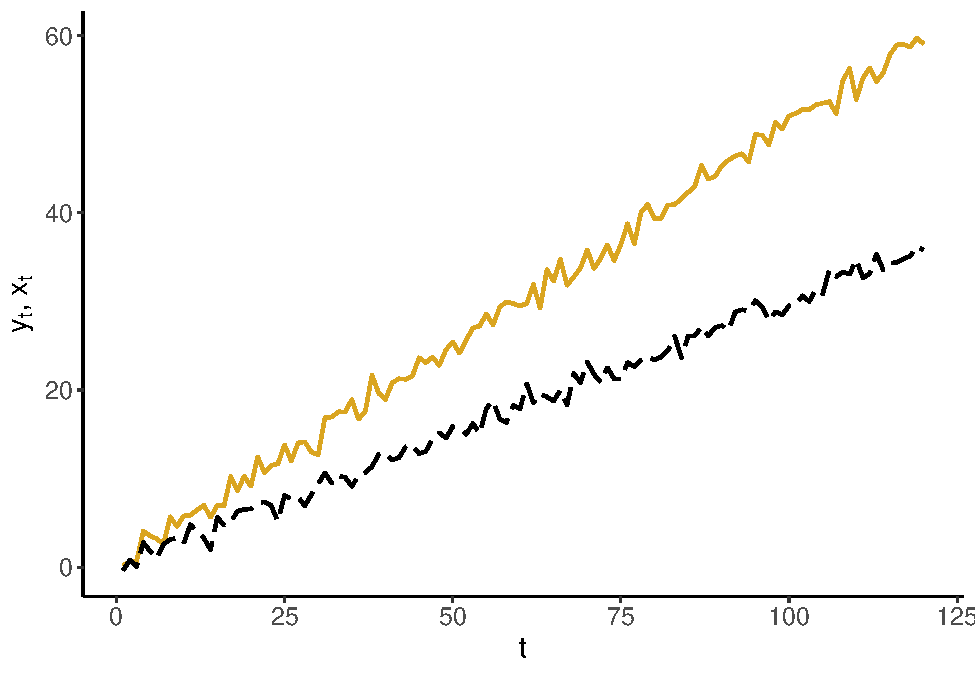
\includegraphics{forecasting_files/figure-latex/unnamed-chunk-6-1.pdf}

If we were to estimate \[y_t = \alpha+\beta x_t + \varepsilon_t,\] we are likely to find the relationship between the two -- in this case \(\beta>0\) -- even though, we know, the two are not related. To illustrate this, we will generate 1000 samples of size 120 for \(y\) and \(x\), and in each case we will estimate the parameter \(\beta\). The following graph illustrates the empirical distribution of these parameter estimates:
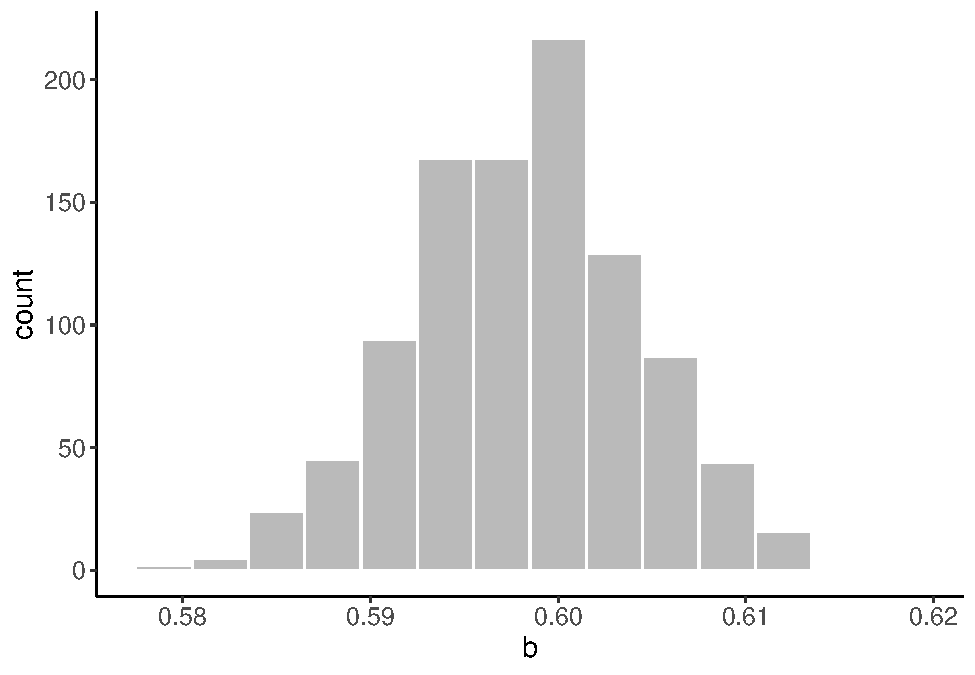
\includegraphics{forecasting_files/figure-latex/unnamed-chunk-7-1.pdf}

Luckily, we can easily ``fix'' the issue, by incorporating a trend in the regression: \[y_t = \alpha+\beta x_t + \eta t + \varepsilon_t.\] Once the trend is accounted for, the previously illustrated ``bias'' disappears. Using a similar simulation exercise as before, the following graph illustrates the empirical distribution of these parameter estimates:
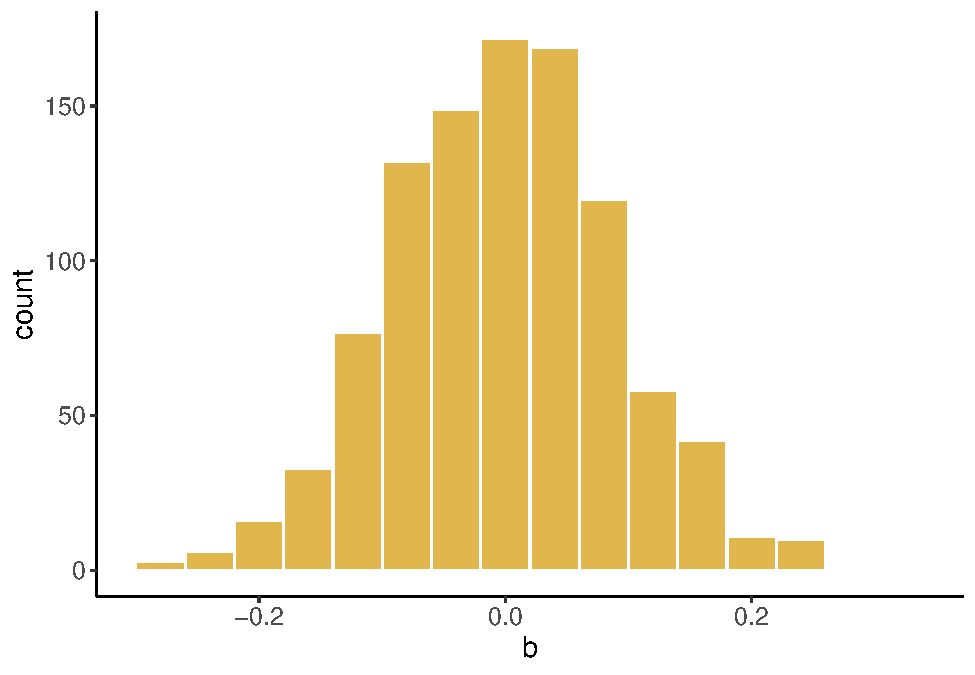
\includegraphics{forecasting_files/figure-latex/unnamed-chunk-8-1.pdf}

In fact, this ``fix'' is equivalent to regressing a de-trended \(y\) on a de-trended \(x\). To de-trend a variable, we first run a regression: \(y_t = \gamma_0 + \gamma_1 t + \nu_t\), and then obtain the fitted values for some fixed trend (typically zero), that is: \(\tilde{y}_t = \hat{\gamma}_0+\hat{\nu}_t\), where \(\hat{\gamma}_0\) and \(\hat{\nu}_t\) are the parameter estimate and the residuals from the foregoing regression.

\hypertarget{modeling}{%
\section{Modeling}\label{modeling}}

As seen, accounting for trends in a time series can help us resolve some regression issues. But a trend in and of itself can be an inherent feature of a times series. To that end, we can apply deterministic trends to forecast time series.

The simplest (and perhaps most frequently applied) model to account for the trending time series is a \emph{linear} trend model: \[y_t = \alpha + \beta t\]

Other likely candidate trend specifications are \emph{polynomial} (e.g.~quadratic, cubic, etc.), \emph{exponential}, and \emph{shifting} (or \emph{switching}) trend models, respectively given by:
\[\begin{aligned}
    y_t &= \alpha + \beta_1 t + \beta_2 t^2 + \ldots + \beta_p t^p \\
    y_t &= e^{\alpha + \beta t}\;~~\mbox{or}\;~~\ln{y_t} = \alpha + \beta t \\
    y_t &= \alpha + \beta_1 t + \beta_2 (t-\tau)I(t>\tau),\;~~\tau\in\mathsf{T} 
    \end{aligned}\]

Of these, here we will primarily consider linear and quadratic trends. An exponential trend, from the standpoint of modeling and forecasting, is equivalent to a linear trend fitted to natural logarithm of the series. For a time series \(\{y_t: t=1,\ldots,T\}\), the natural logarithm is: \(z_t = \ln{y_t}\). Some of the benefits of such a transformation are that:

\begin{itemize}
\tightlist
\item
  they are easier to interpret (relative/percentage change).
\item
  they homogenizes the variance of the time series.
\item
  they may result in improved forecasting accuracy.
\end{itemize}

Exponential trends are suitable when a time series is characterized by a stable relative change over time (e.g., when economic time series grow by 2\% every year).

We will cover the shifting/switching trend models in another chapter.

Trends are (relatively) easy to model and forecast. Caution is needed, however, with (higher order) polynomial trends, as they may fit well in-sample, but cause major problems out-of-sample.

Consider a linear trend model with an additive error term: \[y_t = \alpha + \beta t + \varepsilon_t\] We estimate the model parameters, \(\mathbf{\theta}=\{\alpha,\beta\}\), by fitting the trend model to a time series using the least-squares regression: \[\hat{\theta} = \operatorname*{argmin}_{\mathbf{\theta}} \sum_{t=1}^{T}\big(y_t - \alpha - \beta t\big)^2.\] Fitted values are then given by: \[\hat{y}_t = \hat{\alpha} + \hat{\beta} t\]

\hypertarget{forecasting}{%
\section{Forecasting}\label{forecasting}}

If a linear trend model is fitted to the data, then any future realization of the stochastic process is assumed to follow the linear trend model: \[y_{t+h} = \alpha + \beta (t+h) + \varepsilon_{t+h}.\]

An optimal forecast of \(y_{t+h}\), therefore, is given by: \[y_{t+h|t} = E(y_{t+h}|\Omega_t) = E[\alpha + \beta (t+h) + \varepsilon_{t+h}] = \alpha + \beta (t+h).\]

The forecast error is: \[e_{t+h|t} = y_{t+h} - y_{t+h|t} = \varepsilon_{t+h}\]

The forecast variance, then, is: \[\sigma_{t+h|t}^2 = E(e_{t+h|t}^2) =  E(\varepsilon_{t+h}^2) = \hat{\sigma}^2,\;~~\forall\;h\]

From this, we can obtain interval forecast at any horizon, which is: \[y_{t+h|t} \pm 1.96 \hat{\sigma}.\]

A few features of trend forecasts to note:

\begin{itemize}
\tightlist
\item
  they tend to understate uncertainty (at long horizons as the forecast interval doesn not widen with the horizon);
\item
  short-term trend forecasts can perform poorly; long-term trend forecasts typically perform poorly;
\item
  sometimes it may be beneficial, from the standpoint of achieving better accuracy, to forecast growth rates, and then reconstruct level forecasts.
\end{itemize}

\hypertarget{seasonality}{%
\chapter{Seasonality}\label{seasonality}}

Seasonality is typically modeled as monthly or quarterly pattern, but can also be modeled as a higher frequency pattern (e.g.~weekly). Some examples of time series with apparent seasonal patterns are:

\begin{itemize}
\tightlist
\item
  Agricultural production.
\item
  Sales of energy products.
\item
  Airfare (in non-pandemic times).
\end{itemize}

One way to deal with the seasonality in data is to ``remove'' it prior to the use of the series (i.e., work with a seasonally adjusted time series). Indeed, some economic time series are only/also available in a seasonally-adjusted form.

Otherwise, and perhaps more interestingly, we can directly model seasonality in a regression setting by incorporating seasonal dummy variables.

\hypertarget{modeling-1}{%
\section{Modeling}\label{modeling-1}}

A seasonal model is given by: \[y_t = \sum_{i=1}^{s}\gamma_i d_{it} + \varepsilon_t,\]
where \(s\) denotes the frequency of the data, and \(d_{it}\) takes the value of 1 repeatedly after every \(s\) periods, and such that \(\sum_{i} d_{it} = 1\), \(\forall t\).

Alternatively the seasonal model can be rewritten as: \[y_t = \alpha + \sum_{i=1}^{s-1}\delta_i d_{it} + \varepsilon_t,\] in which case \(\alpha\) is an intercept of an omitted season, and \(\delta_i\) represents a deviation from it during the \(i^{th}\) season.

Both variants of a seasonal model result in an identical fit and forecasts.

\hypertarget{forecasting-1}{%
\section{Forecasting}\label{forecasting-1}}

Any future realization of a random variable that i assumed to follow a seasonal model is: \[y_{t+h} = \alpha + \sum_{i=1}^{s-1}\delta_i d_{i,t+h} + \varepsilon_{t+h}.\]

The optimal forecast of \(y_{t+h}\) is: \[y_{t+h|t} = E(y_{t+h}|\Omega_t) = \alpha + \sum_{i=1}^{s-1}\delta_i d_{i,t+h}\]

The forecast error is: \[e_{t+h|t} = y_{t+h} - y_{t+h|t} = \varepsilon_{t+h}\]

The forecast variance is given by: \[\sigma_{t+h|t}^2 = E(e_{t+h|t}^2) =  E(\varepsilon_{t+h}^2) = \hat{\sigma}^2,\;~~\forall\;h\]

The interval forecast at any horizon is: \[y_{t+h|t} \pm 1.96 \hat{\sigma}.\]

\hypertarget{dynamic-time-series-models}{%
\chapter*{Dynamic Time Series Models}\label{dynamic-time-series-models}}
\addcontentsline{toc}{chapter}{Dynamic Time Series Models}

\hypertarget{linear-autoregression}{%
\chapter{Linear Autoregression}\label{linear-autoregression}}

Economic time series are often characterized by stochastic cycles. A cycle is a pattern of periodic fluctuations, not contained within a calendar year. A stochastic cycle is one generated by random variables. In general terms, the process is given by:
\[Y_t = f(Y_{t-1},Y_{t-2},\ldots;\mathbf{\theta})+\varepsilon_t.\;~~t=1,\ldots,T\]

An autoregressive process (or, simply, an autoregression) is a regression in which the dependent variable and the regressors belong to the same stochastic process.

Autoregression of order \(p\), referred to as \(AR(p)\), has the following functional form:
\[y_t = \alpha + \beta_1 y_{t-1}+\beta_2 y_{t-2}+ \cdots + \beta_p y_{t-p}+\varepsilon_t\]

The sum of the autoregressive parameters, \(\beta_1,\ldots,\beta_p\), depicts the persistence of the series. The larger is the persistence (i.e., closer it is to one), the longer it takes for the effect of a shock to dissolve.

The autocorrelation, \(\rho\), and partial autocorrelation, \(\pi\), functions of the covariance-stationary \(AR(p)\) process have the following distinctive features:

\begin{itemize}
\tightlist
\item
  \(\rho_1 = \pi_1\), and \(\pi_p = \beta_p\).
\item
  The values of \(\beta_1,\ldots,\beta_p\) determine the shape of the autocorrelation function (ACF); in any case, the smaller (in absolute terms) is the persistence measure, the faster the ACF decays toward zero.
\item
  The partial autocorrelation function (PACF) is characterized by ``statistically significant'' first \(p\) spikes \(\pi_1 \neq 0,\ldots,\pi_p \neq 0\), and the remaining \(\pi_k = 0\), \(\forall k > p\).
\end{itemize}

\hypertarget{modeling-2}{%
\section{Modeling}\label{modeling-2}}

\hypertarget{ar1}{%
\subsection{AR(1)}\label{ar1}}

The first-order autoregression is given by: \[y_t = \alpha + \beta_1 y_{t-1} + \varepsilon_t,\] where \(\alpha\) is a constant term; \(\beta_1\) is the \emph{persistence} parameter; and \(\varepsilon_t\) is a white noise process.

A necessary and sufficient condition for an \(AR(1)\) process to be covariance stationary is that \(|\beta_1| < 1\). We can see this by substituting recursively the lagged equations into the lagged dependent variables:
\[
\begin{aligned}
y_t &= \alpha + \beta_1 y_{t-1} + \varepsilon_t \notag \\
y_t &= \alpha + \beta_1 (\alpha + \beta_1 y_{t-2} + \varepsilon_{t-1}) + \varepsilon_t \notag \\
&= \alpha(1+\beta_1) + \beta_1^2 (\alpha + \beta_1 y_{t-3} + \varepsilon_{t-2}) + \beta_1\varepsilon_{t-1} + \varepsilon_t \notag \\
&\vdots  \notag \\
&= \alpha\sum_{i=0}^{k-1}\beta_1^i + \beta_1^k y_{t-k} + \sum_{i=0}^{k-1}\beta_1^i\varepsilon_{t-i}
\end{aligned}
\]
The end-result is a general linear process with geometrically declining coefficients. Here, \(|\beta_1| < 1\) is required for convergence.

Assuming \(|\beta_1| < 1\), as \(k \to \infty\) the process converges to: \[y_t = \frac{\alpha}{1-\beta_1} + \sum_{i=0}^{\infty}\beta_1^i\varepsilon_{t-i}\]

The \emph{unconditional mean} of this process is: \[\mu = E\left(y_t\right) = E\left(\frac{\alpha}{1-\beta_1} + \sum_{i=0}^{\infty}\beta_1^i\varepsilon_{t-i}\right) = \frac{\alpha}{1-\beta_1}\]

The \emph{unconditional variance} of this process is: \[\gamma_0 = Var\left(y_t\right) = Var\left(\frac{\alpha}{1-\beta_1} + \sum_{i=0}^{\infty}\beta_1^i\varepsilon_{t-i}\right) = \frac{\sigma_{\varepsilon}^2}{1-\beta_1^2}\]

The \emph{Autocovariance} is simply the covariance between \(y_t\) and \(y_{t-k}\), that is: \[\gamma_k = Cov(y_t,y_{t-k}) = E[(y_t - \mu)(y_{t-k} - \mu)] = E(y_t y_{t-k}) - \mu^2\]

Some algebraic manipulation can help us show that: \[\gamma_k = \beta_1\gamma_{k-1},\] and that: \[\rho_{k} = \beta_1\rho_{k-1}\] (recall, \emph{autocorrelation} \(\rho_k = \gamma_k/\gamma_0\)).

In fact, for AR(1), the autocorrelation of any order can be given as the autoregression parameter (which in this instance is equivalent to the persistence measure) to that power:
\[
\begin{aligned}
\rho_1 &= \beta_1\rho_0 = \beta_1 \notag \\
\rho_2 &= \beta_1\rho_1 = \beta_1^2 \notag \\
&\vdots \notag \\
\rho_k &= \beta_1\rho_{k-1} = \beta_1^k
\end{aligned}
\]

Thus, the autocorrelation of a covariance stationary AR(1) is a geometric decay; the smaller is \(|\beta_1|\) the more rapid is the decay.

By imposing certain restrictions, the AR(1) will reduce to other already known models:

\begin{itemize}
\tightlist
\item
  If \(\beta_1 = 0\), \(y_t\) is equivalent to a white noise.
\item
  If \(\beta_1 = 1\) and \(\alpha = 0\), \(y_t\) is a random walk.
\item
  If \(\beta_1 = 1\) and \(\alpha \neq 0\), \(y_t\) is a random walk with drift.
\end{itemize}

In general, a smaller persistence parameter results in a quicker adjustment to the \emph{unconditional mean} of the process.

The autocorrelation and partial autocorrelation functions of the AR(1) process have three distinctive features:

\begin{itemize}
\tightlist
\item
  \(\rho_1 = \pi_1 = \beta_1\). That is, the persistence parameter is also the autocorrelation and the partial autocorrelation coefficient.
\item
  The autocorrelation function decreases exponentially toward zero, and the decay is faster when the persistence parameter is smaller.
\item
  The partial autocorrelation function is characterized by only one spike \(\pi_1 \neq 0\), and the remaining \(\pi_k = 0\), \(\forall k > 1\).
\end{itemize}

To illustrate, let's generate a series of 120 observations that follow the process: \(y_t=0.8y_{t-1}+\varepsilon_t\), where \(y_0=0\) and \(\varepsilon\sim N(0,1)\), and plot the ACF and PACF of this series.

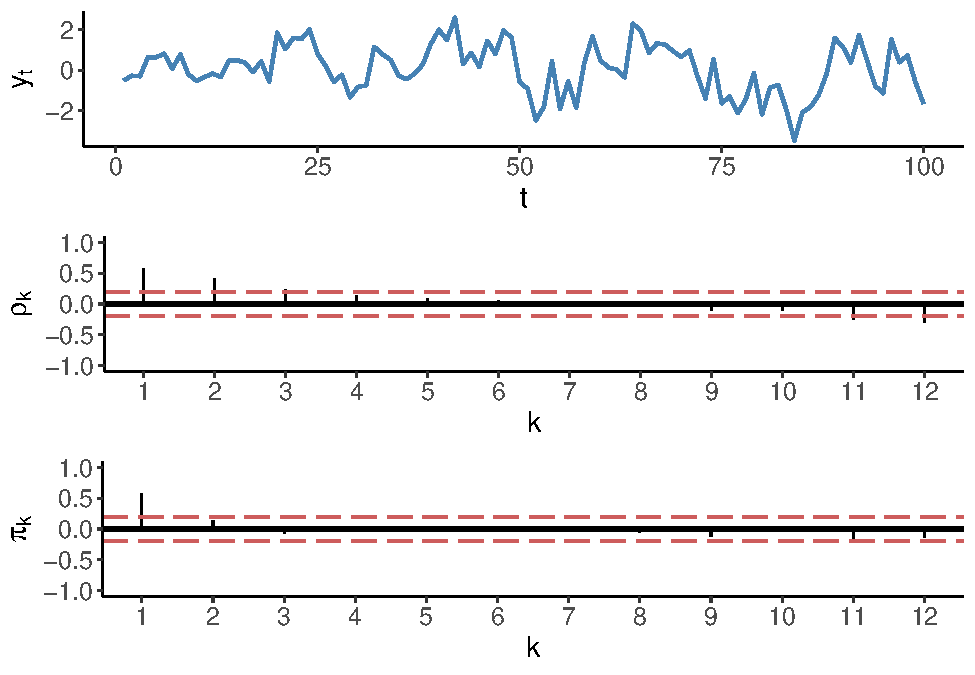
\includegraphics{forecasting_files/figure-latex/unnamed-chunk-10-1.pdf}

\hypertarget{ar2}{%
\subsection{AR(2)}\label{ar2}}

Now consider the second-order autoregression: \[y_t = \alpha + \beta_1 y_{t-1} + \beta_2 y_{t-2} + \varepsilon_t\]

where \(\alpha\) is a constant term; \(\beta_1+\beta_2\) is the persistence measure; and \(\varepsilon_t\) is a white noise process.

In what follows, the necessary (1 and 2) and sufficient (3 and 4) conditions for an \(AR(2)\) process to be covariance stationary are:

\begin{enumerate}
\def\labelenumi{\arabic{enumi}.}
\tightlist
\item
  \(|\beta_2| < 1\)
\item
  \(|\beta_1| < 2\)
\item
  \(\beta_1 + \beta_2 < 1\)
\item
  \(\beta_2 - \beta_1 < 1\)
\end{enumerate}

The autocorrelation functions of the AR(2) process have the following distinctive features:

\begin{itemize}
\tightlist
\item
  \(\rho_1 = \pi_1\) (which is true for any \(AR(p)\) process), and \(\pi_2 = \beta_2\).
\item
  The autocorrelation function decreases toward zero. The path, however, varies depending on the values of \(\beta_1\) and \(\beta_2\). Nonetheless, the decay is faster when the persistence measure is smaller.
\item
  The partial autocorrelation function is characterized by only two spikes \(\pi_1 \neq 0\) and \(\pi_2 \neq 0\), and the remaining \(\pi_k = 0\), \(\forall k > 2\).
\end{itemize}

Again, to illustrate, let's generate a series of 120 observations that follow the process: \(y_t=1.1y_{t-1}-0.4y_{t-2}+\varepsilon_t\), where \(y_{-1}=y_0=0\) and \(\varepsilon\sim N(0,1)\), and plot the ACF and PACF of this series.

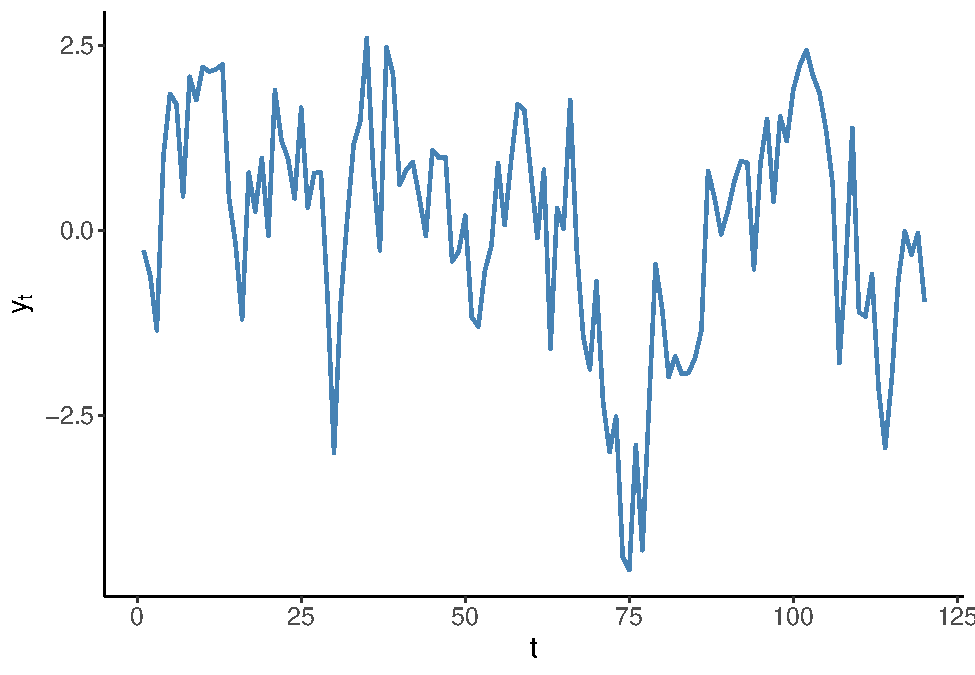
\includegraphics{forecasting_files/figure-latex/unnamed-chunk-11-1.pdf}

\hypertarget{forecasting-2}{%
\section{Forecasting}\label{forecasting-2}}

The optimal one-step-ahead forecast: \[y_{t+1|t} = E(y_{t+1}|\Omega_t) = E(\alpha + \beta_1 y_{t} + \varepsilon_{t+1}) = \alpha + \beta_1 y_{t}\]

The one-step-ahead forecast error: \[e_{t+1|t} = y_{t+1} - y_{t+1|t} = \alpha + \beta_1 y_t + \varepsilon_{t+1} - (\alpha + \beta_1 y_t) = \varepsilon_{t+1}\]

The one-step-ahead forecast variance: \[\sigma_{t+1|t}^2 = Var(y_{t+1}|\Omega_t) = E(e_{t+1|t}^2) = E(\varepsilon_{t+1}^2) = \sigma_{\varepsilon}^2\]

The one-step-ahead (95\%) interval forecast: \[y_{t+1|t} \pm z_{.025}\sigma_{t+1|t} = y_{t+1|t} \pm 1.96\sigma_{\varepsilon}\]

The optimal two-step-ahead forecast: \[y_{t+2|t} = E(y_{t+2}|\Omega_t) = E(\alpha + \beta_1 y_{t+1} + \varepsilon_{t+2}) = \alpha(1+\beta_1) + \beta_1^2 y_t\]

The two-step-ahead forecast error:
\[\begin{aligned}
e_{t+2|t} &= y_{t+2} - y_{t+2|t} \\
&= \alpha(1+\beta_1) + \beta_1^2 y_t + \beta_1\varepsilon_{t+1} + \varepsilon_{t+2} - [\alpha(1+\beta_1) + \beta_1^2 y_t] \\
&= \beta_1\varepsilon_{t+1} + \varepsilon_{t+2}
\end{aligned}\]

The two-step-ahead forecast variance:
\[\begin{aligned}
\sigma_{t+2|t}^2 &= Var(y_{t+2}|\Omega_t) \\
&= E(e_{t+2|t}^2) = E(\beta_1\varepsilon_{t+1} + \varepsilon_{t+2})^2 = \sigma_{\varepsilon}^2(1+\beta_1^2)
\end{aligned}\]

The two-step-ahead (95\%) interval forecast: \[y_{t+2|t} \pm z_{.025}\sigma_{t+2|t} = y_{t+2|t} \pm 1.96\sigma_{\varepsilon}\sqrt{1+\beta_1^2}\]

The optimal h-step-ahead forecast: \[y_{t+h|t} = E(y_{t+h}|\Omega_t) = E(\alpha + \beta_1 y_{t+h-1} + \varepsilon_{t+1}) = \alpha\textstyle\sum_{j=0}^{h-1}\beta_1^j + \beta_1^h y_t\]

The h-step-ahead forecast error: \[e_{t+h|t} = y_{t+h} - y_{t+h|t} = \textstyle\sum_{j=0}^{h-1}\beta_1^j\varepsilon_{t+h-j}\]

The h-step-ahead forecast variance: \[\sigma_{t+h|t}^2 = Var(y_{t+h}|\Omega_t) = E(e_{t+h|t}^2) = \sigma_{\varepsilon}^2\textstyle\sum_{j=0}^{h-1}\beta_1^{2j}\]

The h-step-ahead (95\%) interval forecast: \[y_{t+h|t} \pm z_{.025}\sigma_{t+h|t} = y_{t+1|t} \pm 1.96\sigma_{\varepsilon}\sqrt{\textstyle\sum_{j=0}^{h-1}\beta_1^{2j}}\]

In a covariance-stationary process, i.e.~when \(|\beta_1| < 1\), as \(h \to \infty\):

The optimal point forecast: \[y_{t+h|t} = \frac{\alpha}{1-\beta_1}\]

The forecast variance: \[\sigma_{t+h|t}^2 = \frac{\sigma_{\varepsilon}^2}{1-\beta_1^2}\]

The (95\%) interval forecast: \[y_{t+h|t} \pm z_{.025}\sigma_{t+h|t} = \frac{\alpha}{1-\beta_1} \pm 1.96\frac{\sigma_{\varepsilon}}{\sqrt{1-\beta_1^2}}\]

The optimal one-step-ahead forecast:
\[\begin{aligned}
y_{t+1|t} &= E(y_{t+1}|\Omega_t) \\
&= E(\alpha + \beta_1 y_{t} + \beta_2 y_{t-1} + \varepsilon_{t+1}) = \alpha + \beta_1 y_{t} + \beta_2 y_{t-1}
\end{aligned}\]

The one-step-ahead forecast error:
\[\begin{aligned}
e_{t+1|t} &= y_{t+1} - y_{t+1|t} \\
&= \alpha + \beta_1 y_t + \beta_2 y_{t-1} + \varepsilon_{t+1} - (\alpha + \beta_1 y_t + \beta_2 y_{t-1}) = \varepsilon_{t+1}
\end{aligned}\]

The one-step-ahead forecast variance: \[\sigma_{t+1|t}^2 = Var(y_{t+1}|\Omega_t) = E(e_{t+1|t}^2) = E(\varepsilon_{t+1}^2) = \sigma_{\varepsilon}^2\]

The one-step-ahead (95\%) interval forecast: \[y_{t+1|t} \pm z_{.025}\sigma_{t+1|t} = y_{t+1|t} \pm 1.96\sigma_{\varepsilon}\]

The optimal two-step-ahead forecast:
\[\begin{aligned}
y_{t+2|t} = E(y_{t+2}|\Omega_t) &= E(\alpha + \beta_1 y_{t+1} + \beta_2 y_{t} + \varepsilon_{t+1}) \\
&= \alpha(1+\beta_1) + (\beta_1^2+\beta_2) y_{t} + \beta_1\beta_2 y_{t-1}
\end{aligned}\]

The two-step-ahead forecast error:
\[\begin{aligned}
e_{t+2|t} = y_{t+2} - y_{t+2|t} =& \alpha + \beta_1 y_{t+1} + \beta_2 y_{t} + \varepsilon_{t+2} \\
&- (\alpha + \beta_1 y_{t+1|t} + \beta_2 y_{t}) = \beta_1\varepsilon_{t+1} + \varepsilon_{t+2}
\end{aligned}\]

The two-step-ahead forecast variance:
\[\sigma_{t+2|t}^2 = Var(y_{t+2}|\Omega_t) = E(e_{t+2|t}^2) = E(\beta_1\varepsilon_{t+1} + \varepsilon_{t+2})^2 = \sigma_{\varepsilon}^2(1+\beta_1^2)\]

The two-step-ahead (95\%) interval forecast: \[y_{t+2|t} \pm z_{.025}\sigma_{t+2|t} = y_{t+2|t} \pm 1.96\sigma_{\varepsilon}\sqrt{1+\beta_1^2}\]

The optimal h-step-ahead forecast (iterated method):
\[\begin{aligned}
y_{t+1|t} &= \alpha + \beta_1 y_t + \beta_2 y_{t-1} \\
y_{t+2|t} &= \alpha + \beta_1 y_{t+1|t} + \beta_2 y_{t} \\
y_{t+3|t} &= \alpha + \beta_1 y_{t+2|t} + \beta_2 y_{t+1|t} \\
&\vdots \\
y_{t+h|t} &= \alpha + \beta_1 y_{t+h-1|t} + \beta_2 y_{t+h-2|t}
\end{aligned}\]

The h-step-ahead forecast error: \[e_{t+h|t} = y_{t+h} - y_{t+h|t} = \varepsilon_{t+h}+\beta_1 e_{t+h-1|t}+\beta_2 e_{t+h-2|t}\]

The h-step-ahead forecast variance:
\[\begin{aligned}
\sigma_{t+h|t}^2 &= Var(y_{t+h}|\Omega_t) = E(e_{t+h|t}^2) \\
&= \sigma_{\varepsilon}^2+\beta_1^2 Var(e_{t+h-1|t})+\beta_2^2 Var(e_{t+h-2|t}) \\
&+2\beta_1\beta_2Cov(e_{t+h-1|t},e_{t+h-2|t})
\end{aligned}\]

Note that, in general, formulas for \(\sigma_{t+1|t}^2,\sigma_{t+2|t}^2,\ldots,\sigma_{t+h|t}^2\) are the same for any \(AR(p)\), \(p \geq h-1\).

The h-step-ahead (95\%) interval forecast: \[y_{t+h|t} \pm z_{.025}\sigma_{t+h|t} = y_{t+1|t} \pm 1.96\sigma_{t+h|t}\]

The optimal h-step-ahead forecast: \[y_{t+h|t} = E(y_{t+h}|\Omega_t) = \alpha + \beta_1 y_{t+h-1|t} + \beta_2 y_{t+h-2|t} + \cdots + \beta_p y_{t+h-p|t}\]

The h-step-ahead forecast error: \[e_{t+h|t} = \varepsilon_{t+h} + \beta_1 e_{t+h-1|t} + \beta_2 e_{t+h-2|t} + \cdots + \beta_p e_{t+h-p|t}\]

The h-step-ahead forecast variance:
\[\begin{aligned}
\sigma_{t+h|t}^2 & = Var(y_{t+h}|\Omega_t) = E(e_{t+2|t}^2) \\
&= \sigma_{\varepsilon}^2 + \sum_{i=1}^{p}\beta_i^2 Var(e_{t+h-i|t}) + 2\sum_{i \neq j}\beta_i\beta_j Cov(e_{t+h-i|t},e_{t+h-j|t})
\end{aligned}\]

The h-step-ahead (95\%) interval forecast: \[y_{t+h|t} \pm z_{.025}\sigma_{t+h|t} = y_{t+h|t} \pm 1.96\sigma_{t+h|t}\]

\hypertarget{vector-autoregression}{%
\chapter{Vector Autoregression}\label{vector-autoregression}}

\hypertarget{threshold-autoregression}{%
\chapter{Threshold Autoregression}\label{threshold-autoregression}}

\hypertarget{forecast-assessment}{%
\chapter*{Forecast Assessment}\label{forecast-assessment}}
\addcontentsline{toc}{chapter}{Forecast Assessment}

\hypertarget{forecast-evaluation}{%
\chapter{Forecast Evaluation}\label{forecast-evaluation}}

\hypertarget{forecast-combination}{%
\chapter{Forecast Combination}\label{forecast-combination}}

\hypertarget{introduction-to-r}{%
\chapter*{Introduction to R}\label{introduction-to-r}}
\addcontentsline{toc}{chapter}{Introduction to R}

R is a programming language for data analysis and visualisation. Here I introduce basic commands that should facilitate your understanding of R. You can further enhance your skillset using numerous online resources, as well as your own trial--and--error. To the extent that new features are added to R on a daily basis, there are virtually no limits to how far you can advance your knowledge of this programming language.

We will work in RStudio---the go-to interface for R (as R itself is not an overly user-friendly platform). Thus, you will need to have installed both, R and RStudio on your devise (the latter will `find' and connect with the former on its own). R is available from \href{https://cran.r-project.org/}{CRAN}, and RStudio is available from \href{https://www.rstudio.com/}{RStudio}.

\hypertarget{data-management}{%
\section*{Data Management}\label{data-management}}
\addcontentsline{toc}{section}{Data Management}

There are a number of ways in which we can work with data in R. Let's begin with matrices.

Consider a string of observations:

\begin{Shaded}
\begin{Highlighting}[]
\NormalTok{a }\OtherTok{\textless{}{-}} \FunctionTok{c}\NormalTok{(}\DecValTok{1}\NormalTok{,}\DecValTok{0}\NormalTok{,}\DecValTok{4}\NormalTok{,}\DecValTok{3}\NormalTok{,}\DecValTok{2}\NormalTok{,}\DecValTok{6}\NormalTok{)}
\NormalTok{a}
\end{Highlighting}
\end{Shaded}

\begin{verbatim}
## [1] 1 0 4 3 2 6
\end{verbatim}

A \emph{string}, unlike a \emph{vector}, has no dimensions. But we can transform it to a \(n \times 1\) vector using the as.matrix() function:

\begin{Shaded}
\begin{Highlighting}[]
\NormalTok{b }\OtherTok{\textless{}{-}} \FunctionTok{as.matrix}\NormalTok{(a)}
\NormalTok{b}
\end{Highlighting}
\end{Shaded}

\begin{verbatim}
##      [,1]
## [1,]    1
## [2,]    0
## [3,]    4
## [4,]    3
## [5,]    2
## [6,]    6
\end{verbatim}

The result is a \(6 \times 1\) vector, or a column matrix. To obtain a \(1 \times 6\) vector, or a row matrix, we \emph{transpose} the foregoing vector using the t() function:

\begin{Shaded}
\begin{Highlighting}[]
\NormalTok{bt }\OtherTok{\textless{}{-}} \FunctionTok{t}\NormalTok{(b)}
\NormalTok{bt}
\end{Highlighting}
\end{Shaded}

\begin{verbatim}
##      [,1] [,2] [,3] [,4] [,5] [,6]
## [1,]    1    0    4    3    2    6
\end{verbatim}

\begin{Shaded}
\begin{Highlighting}[]
\FunctionTok{dim}\NormalTok{(bt)}
\end{Highlighting}
\end{Shaded}

\begin{verbatim}
## [1] 1 6
\end{verbatim}

We can create any \(n \times k\) matrix, using the matrix() function. For example, consider a \(3 \times 2\) matrix:

\begin{Shaded}
\begin{Highlighting}[]
\NormalTok{B }\OtherTok{\textless{}{-}} \FunctionTok{matrix}\NormalTok{(a,}\AttributeTok{nrow=}\DecValTok{3}\NormalTok{,}\AttributeTok{ncol=}\DecValTok{2}\NormalTok{)}
\NormalTok{B}
\end{Highlighting}
\end{Shaded}

\begin{verbatim}
##      [,1] [,2]
## [1,]    1    3
## [2,]    0    2
## [3,]    4    6
\end{verbatim}

We can add column names and row names to this matrix:

\begin{Shaded}
\begin{Highlighting}[]
\FunctionTok{colnames}\NormalTok{(B) }\OtherTok{\textless{}{-}} \FunctionTok{c}\NormalTok{(}\StringTok{"c1"}\NormalTok{,}\StringTok{"c2"}\NormalTok{)}
\FunctionTok{rownames}\NormalTok{(B) }\OtherTok{\textless{}{-}} \FunctionTok{c}\NormalTok{(}\StringTok{"r1"}\NormalTok{,}\StringTok{"r2"}\NormalTok{,}\StringTok{"r3"}\NormalTok{)}
\NormalTok{B}
\end{Highlighting}
\end{Shaded}

\begin{verbatim}
##    c1 c2
## r1  1  3
## r2  0  2
## r3  4  6
\end{verbatim}

If, at this point, we would like to only work with, say, the first column of the matrix, we can call it using its column number, (1), or the column name, (``c1''), as follows:

\begin{Shaded}
\begin{Highlighting}[]
\NormalTok{B[,}\StringTok{"c1"}\NormalTok{]}
\end{Highlighting}
\end{Shaded}

\begin{verbatim}
## r1 r2 r3 
##  1  0  4
\end{verbatim}

Similarly, if we want to refer to a matrix element, say \(b_{3,2}\), we can do this as follows:

\begin{Shaded}
\begin{Highlighting}[]
\NormalTok{B[}\DecValTok{3}\NormalTok{,}\DecValTok{2}\NormalTok{]}
\end{Highlighting}
\end{Shaded}

\begin{verbatim}
## [1] 6
\end{verbatim}

Matrix multiplication is done using \%*\% command, granted that the two matrices are compatible. For example, we obtain a product of matrix \(B\) and a new \(2 \times 1\) vector, \(d\), as follows:

\begin{Shaded}
\begin{Highlighting}[]
\NormalTok{d }\OtherTok{\textless{}{-}} \FunctionTok{as.matrix}\NormalTok{(}\FunctionTok{c}\NormalTok{(}\DecValTok{5}\NormalTok{,}\SpecialCharTok{{-}}\DecValTok{2}\NormalTok{))}
\NormalTok{Bd }\OtherTok{\textless{}{-}}\NormalTok{ B}\SpecialCharTok{\%*\%}\NormalTok{d}
\NormalTok{Bd}
\end{Highlighting}
\end{Shaded}

\begin{verbatim}
##    [,1]
## r1   -1
## r2   -4
## r3    8
\end{verbatim}

We can add columns (and rows) to the existing matrix using a cbind() function:

\begin{Shaded}
\begin{Highlighting}[]
\NormalTok{c3 }\OtherTok{\textless{}{-}} \FunctionTok{c}\NormalTok{(}\DecValTok{0}\NormalTok{,}\DecValTok{1}\NormalTok{,}\DecValTok{0}\NormalTok{)}
\NormalTok{D }\OtherTok{\textless{}{-}} \FunctionTok{cbind}\NormalTok{(B,c3)}
\NormalTok{D}
\end{Highlighting}
\end{Shaded}

\begin{verbatim}
##    c1 c2 c3
## r1  1  3  0
## r2  0  2  1
## r3  4  6  0
\end{verbatim}

We can invert a(n invertible) matrix using the solve() function:

\begin{Shaded}
\begin{Highlighting}[]
\NormalTok{Di }\OtherTok{\textless{}{-}} \FunctionTok{solve}\NormalTok{(D)}
\NormalTok{Di}
\end{Highlighting}
\end{Shaded}

\begin{verbatim}
##            r1 r2         r3
## c1 -1.0000000  0  0.5000000
## c2  0.6666667  0 -0.1666667
## c3 -1.3333333  1  0.3333333
\end{verbatim}

\hypertarget{data-visualisation}{%
\section*{Data Visualisation}\label{data-visualisation}}
\addcontentsline{toc}{section}{Data Visualisation}

One of the comparative advantages of R is in its graphing aesthetics. Currently, the best graphs are plotted via the \textbf{ggplot2} package. Notably, this package requires that the data are maintained in the data.frame or the data.table format (for the latter, you need to load the \textbf{data.table} package). Let's create a data.table object and observe its few lines:

\begin{Shaded}
\begin{Highlighting}[]
\FunctionTok{set.seed}\NormalTok{(}\DecValTok{1}\NormalTok{)}
\NormalTok{x }\OtherTok{\textless{}{-}} \FunctionTok{runif}\NormalTok{(}\DecValTok{120}\NormalTok{,}\DecValTok{0}\NormalTok{,}\DecValTok{2}\NormalTok{)}
\NormalTok{y }\OtherTok{\textless{}{-}} \FloatTok{0.2+0.7}\SpecialCharTok{*}\NormalTok{x}\SpecialCharTok{+}\FunctionTok{rnorm}\NormalTok{(}\DecValTok{120}\NormalTok{)}

\FunctionTok{library}\NormalTok{(data.table)}

\NormalTok{dt }\OtherTok{\textless{}{-}} \FunctionTok{data.table}\NormalTok{(}\AttributeTok{y=}\NormalTok{y,}\AttributeTok{x=}\NormalTok{x)}
\NormalTok{dt}
\end{Highlighting}
\end{Shaded}

\begin{verbatim}
##               y          x
##   1:  2.9733299 0.53101733
##   2:  0.6817335 0.74424780
##   3:  1.6917341 1.14570673
##   4:  1.4994931 1.81641558
##   5: -0.2609185 0.40336386
##  ---                      
## 116:  0.1835826 0.02615515
## 117:  1.9894321 1.43113213
## 118:  2.4197029 0.20636847
## 119:  1.8521905 0.89256870
## 120:  2.3040499 1.28020209
\end{verbatim}

Now, let's load \textbf{ggplot2} and generate a simple scatter plot:

\begin{Shaded}
\begin{Highlighting}[]
\FunctionTok{library}\NormalTok{(ggplot2)}

\FunctionTok{ggplot}\NormalTok{(dt,}\FunctionTok{aes}\NormalTok{(}\AttributeTok{x=}\NormalTok{x,}\AttributeTok{y=}\NormalTok{y))}\SpecialCharTok{+}
  \FunctionTok{geom\_point}\NormalTok{()}
\end{Highlighting}
\end{Shaded}

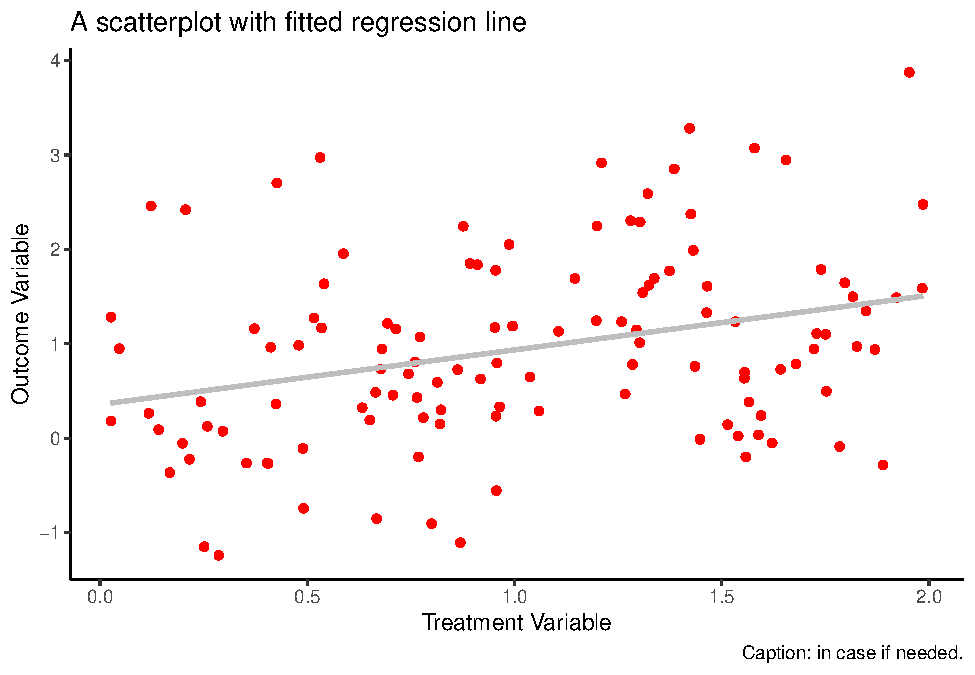
\includegraphics{forecasting_files/figure-latex/unnamed-chunk-28-1.pdf}

We can augment this plot in a number of different ways. Here we change the point color to red, add the fitted regression line to the plot, add labels to the figure, and apply a `classic' background theme:

\begin{Shaded}
\begin{Highlighting}[]
\FunctionTok{ggplot}\NormalTok{(dt,}\FunctionTok{aes}\NormalTok{(}\AttributeTok{x=}\NormalTok{x,}\AttributeTok{y=}\NormalTok{y))}\SpecialCharTok{+}
  \FunctionTok{geom\_point}\NormalTok{(}\AttributeTok{color=}\StringTok{"goldenrod"}\NormalTok{)}\SpecialCharTok{+}
  \FunctionTok{geom\_smooth}\NormalTok{(}\AttributeTok{method=}\StringTok{"lm"}\NormalTok{,}\AttributeTok{formula=}\NormalTok{y}\SpecialCharTok{\textasciitilde{}}\NormalTok{x,}\AttributeTok{se=}\NormalTok{F,}\AttributeTok{color=}\StringTok{"darkgray"}\NormalTok{)}\SpecialCharTok{+}
  \FunctionTok{labs}\NormalTok{(}\AttributeTok{title=}\StringTok{"A scatterplot with fitted regression line"}\NormalTok{, }
       \AttributeTok{x=}\StringTok{"Treatment Variable"}\NormalTok{, }
       \AttributeTok{y=}\StringTok{"Outcome Variable"}\NormalTok{, }
       \AttributeTok{caption=}\StringTok{"Caption: in case if needed."}\NormalTok{)}\SpecialCharTok{+}
  \FunctionTok{theme\_classic}\NormalTok{()}
\end{Highlighting}
\end{Shaded}

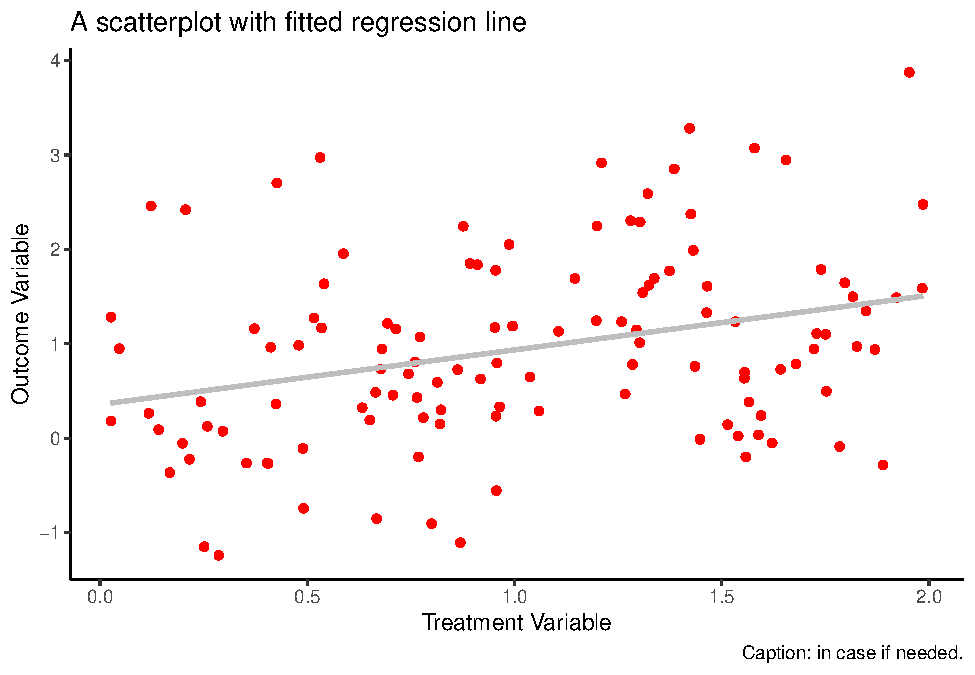
\includegraphics{forecasting_files/figure-latex/unnamed-chunk-29-1.pdf}

As another example, let's generate a histogram (of the dependent variable):

\begin{Shaded}
\begin{Highlighting}[]
\FunctionTok{ggplot}\NormalTok{(dt,}\FunctionTok{aes}\NormalTok{(}\AttributeTok{x=}\NormalTok{y))}\SpecialCharTok{+}
  \FunctionTok{geom\_histogram}\NormalTok{(}\AttributeTok{color=}\StringTok{"white"}\NormalTok{,}\AttributeTok{fill=}\StringTok{"goldenrod"}\NormalTok{,}\AttributeTok{binwidth=}\NormalTok{.}\DecValTok{5}\NormalTok{)}\SpecialCharTok{+}
  \FunctionTok{labs}\NormalTok{(}\AttributeTok{title=}\StringTok{"A basic histogram"}\NormalTok{)}\SpecialCharTok{+}
  \FunctionTok{theme\_classic}\NormalTok{()}
\end{Highlighting}
\end{Shaded}

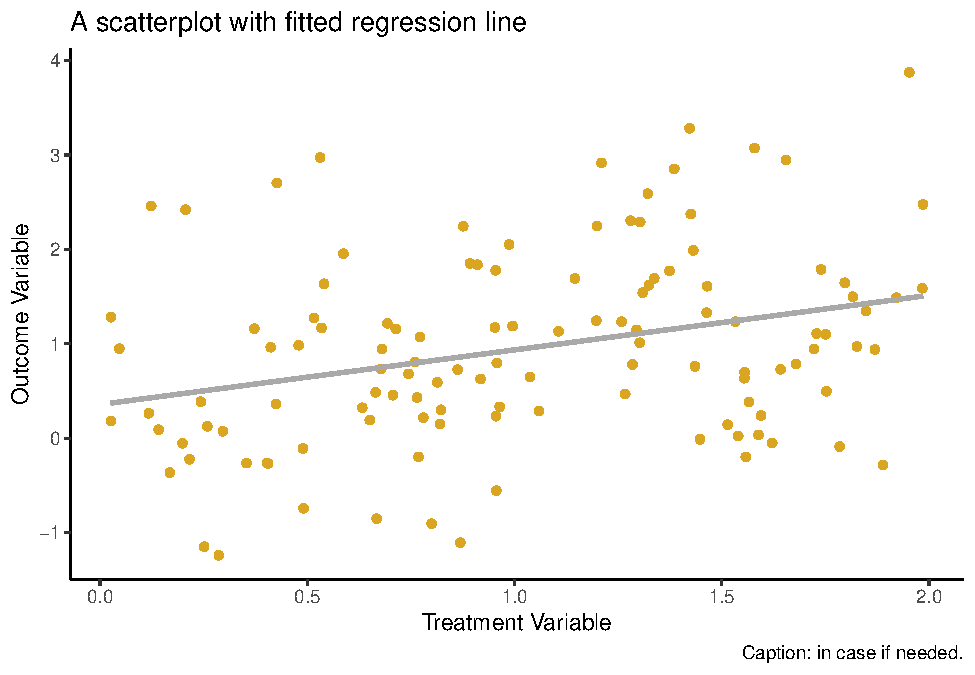
\includegraphics{forecasting_files/figure-latex/unnamed-chunk-30-1.pdf}

We typically apply a line plot to illustrate a time series (that are ordered by date). In what follows, we add a date column to our data frame and then plot the dependent variable in the chronological order:

\begin{Shaded}
\begin{Highlighting}[]
\NormalTok{dt}\SpecialCharTok{$}\NormalTok{date }\OtherTok{\textless{}{-}} \FunctionTok{seq}\NormalTok{(}\AttributeTok{from=}\FunctionTok{as.Date}\NormalTok{(}\StringTok{"2000{-}01{-}01"}\NormalTok{),}\AttributeTok{by=}\StringTok{"month"}\NormalTok{,}\AttributeTok{along.with=}\NormalTok{y)}

\FunctionTok{ggplot}\NormalTok{(dt,}\FunctionTok{aes}\NormalTok{(}\AttributeTok{x=}\NormalTok{date,}\AttributeTok{y=}\NormalTok{y))}\SpecialCharTok{+}
  \FunctionTok{geom\_line}\NormalTok{(}\AttributeTok{color=}\StringTok{"goldenrod"}\NormalTok{)}\SpecialCharTok{+}
  \FunctionTok{labs}\NormalTok{(}\AttributeTok{title=}\StringTok{"A basic time series plot"}\NormalTok{,  }
       \AttributeTok{x=}\StringTok{"Year"}\NormalTok{, }
       \AttributeTok{y=}\StringTok{"Outcome Variable"}\NormalTok{)}\SpecialCharTok{+}
  \FunctionTok{theme\_classic}\NormalTok{()}
\end{Highlighting}
\end{Shaded}

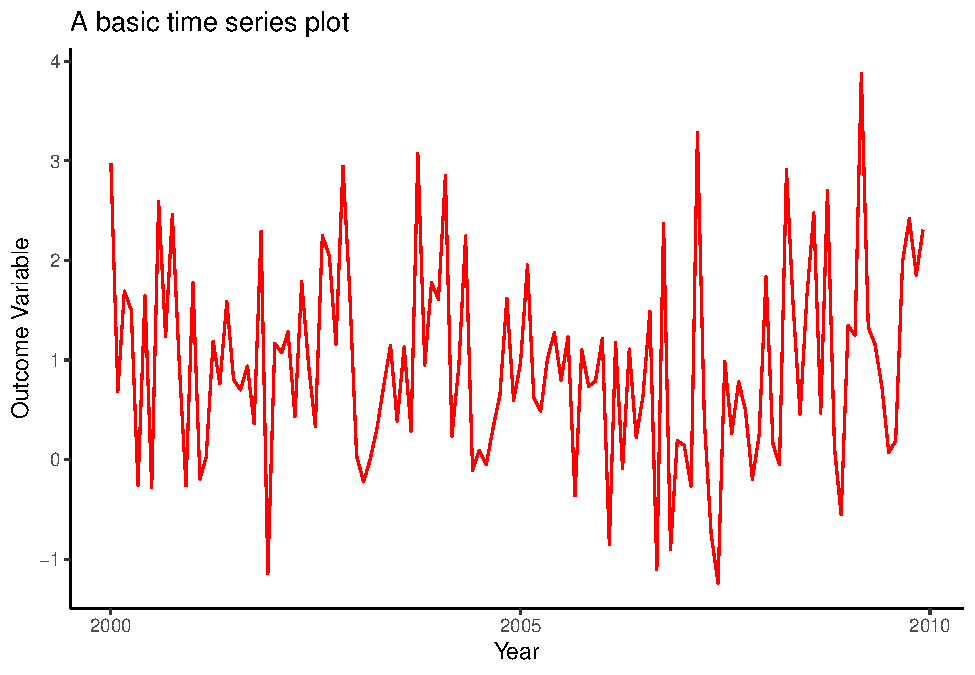
\includegraphics{forecasting_files/figure-latex/unnamed-chunk-31-1.pdf}

\hypertarget{regression-analysis}{%
\section*{Regression Analysis}\label{regression-analysis}}
\addcontentsline{toc}{section}{Regression Analysis}

To illustrate the OLS regression in R, we apply the previously generated \(x\) and \(y\) as independent and dependent variables. To begin, we obtain the least squares estimator ``by hand'' as follows:

\begin{Shaded}
\begin{Highlighting}[]
\NormalTok{X }\OtherTok{\textless{}{-}} \FunctionTok{cbind}\NormalTok{(}\DecValTok{1}\NormalTok{,x)}
\NormalTok{b }\OtherTok{\textless{}{-}} \FunctionTok{solve}\NormalTok{(}\FunctionTok{t}\NormalTok{(X)}\SpecialCharTok{\%*\%}\NormalTok{X)}\SpecialCharTok{\%*\%}\FunctionTok{t}\NormalTok{(X)}\SpecialCharTok{\%*\%}\NormalTok{y}
\NormalTok{b}
\end{Highlighting}
\end{Shaded}

\begin{verbatim}
##        [,1]
##   0.3577680
## x 0.5781188
\end{verbatim}

This can be easily done using the lm() function:

\begin{Shaded}
\begin{Highlighting}[]
\NormalTok{ols }\OtherTok{\textless{}{-}} \FunctionTok{lm}\NormalTok{(y}\SpecialCharTok{\textasciitilde{}}\NormalTok{x)}
\NormalTok{ols}
\end{Highlighting}
\end{Shaded}

\begin{verbatim}
## 
## Call:
## lm(formula = y ~ x)
## 
## Coefficients:
## (Intercept)            x  
##      0.3578       0.5781
\end{verbatim}

We can apply the summary() function to see the complete set of regression results:

\begin{Shaded}
\begin{Highlighting}[]
\FunctionTok{summary}\NormalTok{(ols)}
\end{Highlighting}
\end{Shaded}

\begin{verbatim}
## 
## Call:
## lm(formula = y ~ x)
## 
## Residuals:
##     Min      1Q  Median      3Q     Max 
## -1.9662 -0.5983 -0.1127  0.5639  2.3882 
## 
## Coefficients:
##             Estimate Std. Error t value Pr(>|t|)    
## (Intercept)   0.3578     0.1904   1.879 0.062717 .  
## x             0.5781     0.1641   3.522 0.000609 ***
## ---
## Signif. codes:  0 '***' 0.001 '**' 0.01 '*' 0.05 '.' 0.1 ' ' 1
## 
## Residual standard error: 0.9716 on 118 degrees of freedom
## Multiple R-squared:  0.09514,    Adjusted R-squared:  0.08748 
## F-statistic: 12.41 on 1 and 118 DF,  p-value: 0.0006091
\end{verbatim}

\hypertarget{tutorial-1}{%
\chapter*{Tutorial 1}\label{tutorial-1}}
\addcontentsline{toc}{chapter}{Tutorial 1}

In this tutorial, we will introduce several simple R functions, and will perform a basic forecasting exercise.

Let's generate a sequence of 200 iid random variables with mean zero and variance 4, call it e.

\begin{Shaded}
\begin{Highlighting}[]
\FunctionTok{set.seed}\NormalTok{(}\DecValTok{1}\NormalTok{)}
\NormalTok{e }\OtherTok{\textless{}{-}} \FunctionTok{rnorm}\NormalTok{(}\DecValTok{200}\NormalTok{,}\DecValTok{0}\NormalTok{,}\DecValTok{2}\NormalTok{)}
\end{Highlighting}
\end{Shaded}

Notice that prior to sampling we set seed to some value (to one in this instance). We do so to ensure that we can exactly replicate the sample in the future.

Nett, generate a sequence of 200 binary variables, call it x.

\begin{Shaded}
\begin{Highlighting}[]
\FunctionTok{set.seed}\NormalTok{(}\DecValTok{2}\NormalTok{)}
\NormalTok{x }\OtherTok{\textless{}{-}} \FunctionTok{sample}\NormalTok{(}\FunctionTok{c}\NormalTok{(}\DecValTok{0}\NormalTok{,}\DecValTok{1}\NormalTok{),}\DecValTok{200}\NormalTok{,}\AttributeTok{replace=}\NormalTok{T)}
\end{Highlighting}
\end{Shaded}

Construct a dependent variable, y, using the following formula: \(y=2+0.5x+e\).

\begin{Shaded}
\begin{Highlighting}[]
\NormalTok{y }\OtherTok{\textless{}{-}} \DecValTok{2}\FloatTok{+0.5}\SpecialCharTok{*}\NormalTok{x}\SpecialCharTok{+}\NormalTok{e}
\end{Highlighting}
\end{Shaded}

Regress y on x, using the \texttt{lm()} function, to obtain estimates of the intercept and slope parameters.

\begin{Shaded}
\begin{Highlighting}[]
\NormalTok{ols }\OtherTok{\textless{}{-}} \FunctionTok{lm}\NormalTok{(y}\SpecialCharTok{\textasciitilde{}}\NormalTok{x)}
\NormalTok{ols}
\end{Highlighting}
\end{Shaded}

\begin{verbatim}
## 
## Call:
## lm(formula = y ~ x)
## 
## Coefficients:
## (Intercept)            x  
##      2.1244       0.3854
\end{verbatim}

Generate some ``future'' realizations (100 observations) of y.

\begin{Shaded}
\begin{Highlighting}[]
\FunctionTok{set.seed}\NormalTok{(}\DecValTok{3}\NormalTok{)}
\NormalTok{e }\OtherTok{\textless{}{-}} \FunctionTok{rnorm}\NormalTok{(}\DecValTok{100}\NormalTok{,}\DecValTok{0}\NormalTok{,}\DecValTok{2}\NormalTok{)}

\FunctionTok{set.seed}\NormalTok{(}\DecValTok{4}\NormalTok{)}
\NormalTok{x }\OtherTok{\textless{}{-}} \FunctionTok{sample}\NormalTok{(}\FunctionTok{c}\NormalTok{(}\DecValTok{0}\NormalTok{,}\DecValTok{1}\NormalTok{),}\DecValTok{100}\NormalTok{,}\AttributeTok{replace=}\NormalTok{T)}

\NormalTok{y }\OtherTok{\textless{}{-}} \DecValTok{2}\FloatTok{+0.5}\SpecialCharTok{*}\NormalTok{x}\SpecialCharTok{+}\NormalTok{e}
\end{Highlighting}
\end{Shaded}

Note that these represent actual realizations of the variable; these not forecasts.

Suppose we think that in the considered forecast period, x only takes on 1 (below we will refer to this as the Model 1). Based on this, and using parameter estimates from above, let's generate forecasts for this period.

\begin{Shaded}
\begin{Highlighting}[]
\NormalTok{y\_f1 }\OtherTok{\textless{}{-}}\NormalTok{ ols}\SpecialCharTok{$}\NormalTok{coefficients[}\DecValTok{1}\NormalTok{]}\SpecialCharTok{+}\NormalTok{ols}\SpecialCharTok{$}\NormalTok{coefficients[}\DecValTok{2}\NormalTok{]}\SpecialCharTok{*}\FunctionTok{rep}\NormalTok{(}\DecValTok{1}\NormalTok{,}\DecValTok{100}\NormalTok{)}
\end{Highlighting}
\end{Shaded}

At this point, we have actual realisations of y and its forecasts. Thus, we can obtain forecast errors, mean absolute forecast errors, and root mean square forecast errors.

\begin{Shaded}
\begin{Highlighting}[]
\NormalTok{e\_f1 }\OtherTok{\textless{}{-}}\NormalTok{ y}\SpecialCharTok{{-}}\NormalTok{y\_f1}

\NormalTok{mafe1 }\OtherTok{\textless{}{-}} \FunctionTok{mean}\NormalTok{(}\FunctionTok{abs}\NormalTok{(e\_f1))}
\NormalTok{rmsfe1 }\OtherTok{\textless{}{-}} \FunctionTok{sqrt}\NormalTok{(}\FunctionTok{mean}\NormalTok{(e\_f1}\SpecialCharTok{\^{}}\DecValTok{2}\NormalTok{))}

\NormalTok{mafe1}
\end{Highlighting}
\end{Shaded}

\begin{verbatim}
## [1] 1.43523
\end{verbatim}

\begin{Shaded}
\begin{Highlighting}[]
\NormalTok{rmsfe1}
\end{Highlighting}
\end{Shaded}

\begin{verbatim}
## [1] 1.739508
\end{verbatim}

Suppose, instead, we think that in the considered forecast period x only takes on 0 (below we will refer to this as the Model 2). Based on this, and using parameter estimates from above, let's generate forecasts for this period.

\begin{Shaded}
\begin{Highlighting}[]
\NormalTok{y\_f0 }\OtherTok{\textless{}{-}}\NormalTok{ ols}\SpecialCharTok{$}\NormalTok{coefficients[}\DecValTok{1}\NormalTok{]}\SpecialCharTok{+}\NormalTok{ols}\SpecialCharTok{$}\NormalTok{coefficients[}\DecValTok{2}\NormalTok{]}\SpecialCharTok{*}\FunctionTok{rep}\NormalTok{(}\DecValTok{0}\NormalTok{,}\DecValTok{100}\NormalTok{)}
\end{Highlighting}
\end{Shaded}

Using these forecasts, obtain forecast errors, mean absolute forecast errors, and root mean square forecast errors.

\begin{Shaded}
\begin{Highlighting}[]
\NormalTok{e\_f0 }\OtherTok{\textless{}{-}}\NormalTok{ y}\SpecialCharTok{{-}}\NormalTok{y\_f0}

\NormalTok{mafe0 }\OtherTok{\textless{}{-}} \FunctionTok{mean}\NormalTok{(}\FunctionTok{abs}\NormalTok{(e\_f0))}
\NormalTok{rmsfe0 }\OtherTok{\textless{}{-}} \FunctionTok{sqrt}\NormalTok{(}\FunctionTok{mean}\NormalTok{(e\_f0}\SpecialCharTok{\^{}}\DecValTok{2}\NormalTok{))}

\NormalTok{mafe0}
\end{Highlighting}
\end{Shaded}

\begin{verbatim}
## [1] 1.455768
\end{verbatim}

\begin{Shaded}
\begin{Highlighting}[]
\NormalTok{rmsfe0}
\end{Highlighting}
\end{Shaded}

\begin{verbatim}
## [1] 1.736182
\end{verbatim}

By comparing the two sets of forecasts, we can observe a somewhat rare and yet not an unlikely scenario: MAFE points to the Model 1 as more accurate of the two models, while RMSFE suggests the Model 2 as the more accurate one. More often than not, however, these two accuracy measures tend to agree.

\hypertarget{tutorial-2}{%
\chapter*{Tutorial 2}\label{tutorial-2}}
\addcontentsline{toc}{chapter}{Tutorial 2}

In this tutorial, we will introduce `for loop,' and use it to generate time series as well as to obtain one-step-ahead forecasts using a rolling window procedure; we will also perform forecast error diagnostics.

Let's generate a random walk process, such that \(y_{t} = y_{t-1}+e_{t}\), where \(e_{t} ~ N(0,1)\), and where \(y_{0}=0\), for \(t=1,\ldots,120\).

\begin{Shaded}
\begin{Highlighting}[]
\NormalTok{n }\OtherTok{\textless{}{-}} \DecValTok{120}

\FunctionTok{set.seed}\NormalTok{(}\DecValTok{1}\NormalTok{)}
\NormalTok{e }\OtherTok{\textless{}{-}} \FunctionTok{rnorm}\NormalTok{(n)}

\NormalTok{y }\OtherTok{\textless{}{-}} \FunctionTok{rep}\NormalTok{(}\ConstantTok{NA}\NormalTok{,n)}

\NormalTok{y[}\DecValTok{1}\NormalTok{] }\OtherTok{\textless{}{-}}\NormalTok{ e[}\DecValTok{1}\NormalTok{]}

\ControlFlowTok{for}\NormalTok{(i }\ControlFlowTok{in} \DecValTok{2}\SpecialCharTok{:}\NormalTok{n)\{}
\NormalTok{  y[i] }\OtherTok{\textless{}{-}}\NormalTok{ y[i}\DecValTok{{-}1}\NormalTok{] }\SpecialCharTok{+}\NormalTok{ e[i]}
\NormalTok{\}}
\end{Highlighting}
\end{Shaded}

Store \(y\) and \(e\) in a \textbf{data.table}, call it `dt.' Add some arbitrary dates to the data (e.g., suppose we deal with the monthly series beginning from January 2011).

\begin{Shaded}
\begin{Highlighting}[]
\NormalTok{dt }\OtherTok{\textless{}{-}} \FunctionTok{data.table}\NormalTok{(y,e)}

\NormalTok{dt}\SpecialCharTok{$}\NormalTok{date }\OtherTok{\textless{}{-}} \FunctionTok{seq}\NormalTok{(}\FunctionTok{as.Date}\NormalTok{(}\StringTok{"2011{-}01{-}01"}\NormalTok{),}\FunctionTok{as.Date}\NormalTok{(}\StringTok{"2020{-}12{-}01"}\NormalTok{),}\AttributeTok{by=}\StringTok{"month"}\NormalTok{)}
\end{Highlighting}
\end{Shaded}

Plot the realized time series using \textbf{ggplot} function.

\begin{Shaded}
\begin{Highlighting}[]
\FunctionTok{ggplot}\NormalTok{(dt,}\FunctionTok{aes}\NormalTok{(}\AttributeTok{x=}\NormalTok{date,}\AttributeTok{y=}\NormalTok{y))}\SpecialCharTok{+}
  \FunctionTok{geom\_line}\NormalTok{(}\AttributeTok{size=}\DecValTok{1}\NormalTok{)}\SpecialCharTok{+}
  \FunctionTok{labs}\NormalTok{(}\AttributeTok{x=}\StringTok{"Year"}\NormalTok{,}\AttributeTok{y=}\StringTok{"Random Walk"}\NormalTok{)}\SpecialCharTok{+}
  \FunctionTok{theme\_classic}\NormalTok{()}
\end{Highlighting}
\end{Shaded}

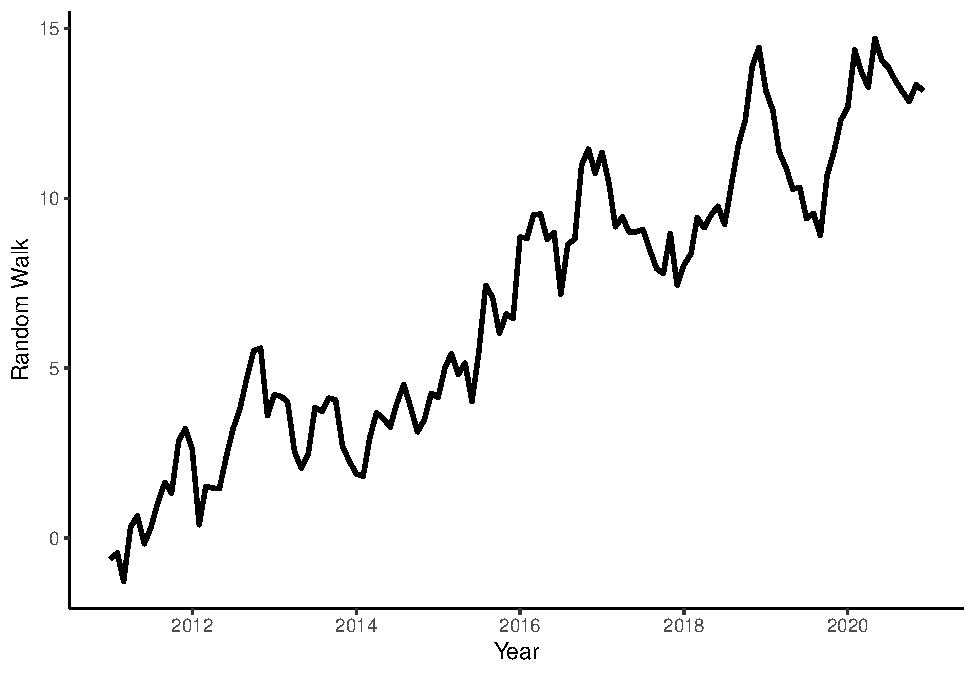
\includegraphics{forecasting_files/figure-latex/unnamed-chunk-48-1.pdf}

Generate a sequence of one-step-ahead forecasts from naive and average methods, using the rolling window scheme, where the first rolling window ranges from period 1 to period 80.

\begin{Shaded}
\begin{Highlighting}[]
\NormalTok{dt}\SpecialCharTok{$}\NormalTok{average }\OtherTok{\textless{}{-}} \ConstantTok{NA}
\NormalTok{dt}\SpecialCharTok{$}\NormalTok{naive }\OtherTok{\textless{}{-}} \ConstantTok{NA}

\NormalTok{R }\OtherTok{\textless{}{-}} \DecValTok{80}
\NormalTok{P }\OtherTok{\textless{}{-}}\NormalTok{ n}\SpecialCharTok{{-}}\NormalTok{R}
\ControlFlowTok{for}\NormalTok{(i }\ControlFlowTok{in} \DecValTok{1}\SpecialCharTok{:}\NormalTok{P)\{}
\NormalTok{  w }\OtherTok{\textless{}{-}}\NormalTok{ y[i}\SpecialCharTok{:}\NormalTok{(R}\DecValTok{{-}1}\SpecialCharTok{+}\NormalTok{i)]}
\NormalTok{  dt}\SpecialCharTok{$}\NormalTok{average[R}\SpecialCharTok{+}\NormalTok{i] }\OtherTok{\textless{}{-}} \FunctionTok{mean}\NormalTok{(w)}
\NormalTok{  dt}\SpecialCharTok{$}\NormalTok{naive[R}\SpecialCharTok{+}\NormalTok{i] }\OtherTok{\textless{}{-}}\NormalTok{ w[}\FunctionTok{length}\NormalTok{(w)]}
\NormalTok{\}}
\end{Highlighting}
\end{Shaded}

Calculate the RMSFE measures for each of the two forecasting methods.

\begin{Shaded}
\begin{Highlighting}[]
\NormalTok{dt[,}\StringTok{\textasciigrave{}}\AttributeTok{:=}\StringTok{\textasciigrave{}}\NormalTok{(}\AttributeTok{e\_average=}\NormalTok{y}\SpecialCharTok{{-}}\NormalTok{average,}\AttributeTok{e\_naive=}\NormalTok{y}\SpecialCharTok{{-}}\NormalTok{naive)]}

\NormalTok{rmsfe\_average }\OtherTok{\textless{}{-}} \FunctionTok{sqrt}\NormalTok{(}\FunctionTok{mean}\NormalTok{(dt}\SpecialCharTok{$}\NormalTok{e\_average}\SpecialCharTok{\^{}}\DecValTok{2}\NormalTok{,}\AttributeTok{na.rm=}\NormalTok{T))}
\NormalTok{rmsfe\_naive }\OtherTok{\textless{}{-}} \FunctionTok{sqrt}\NormalTok{(}\FunctionTok{mean}\NormalTok{(dt}\SpecialCharTok{$}\NormalTok{e\_naive}\SpecialCharTok{\^{}}\DecValTok{2}\NormalTok{,}\AttributeTok{na.rm=}\NormalTok{T))}

\NormalTok{rmsfe\_average}
\end{Highlighting}
\end{Shaded}

\begin{verbatim}
## [1] 4.672947
\end{verbatim}

\begin{Shaded}
\begin{Highlighting}[]
\NormalTok{rmsfe\_naive}
\end{Highlighting}
\end{Shaded}

\begin{verbatim}
## [1] 0.850081
\end{verbatim}

Perform the forecast error diagnostics for the two considered methods.

Zero mean of the forecast errors: \(E(e_{t+1|t})=0\).
We perform this test by regressing the forecast error on the constant, and checking whether the coefficient is statistically significantly different from zero.

\begin{Shaded}
\begin{Highlighting}[]
\FunctionTok{summary}\NormalTok{(}\FunctionTok{lm}\NormalTok{(e\_average}\SpecialCharTok{\textasciitilde{}}\DecValTok{1}\NormalTok{,}\AttributeTok{data=}\NormalTok{dt))}\SpecialCharTok{$}\NormalTok{coefficients}
\end{Highlighting}
\end{Shaded}

\begin{verbatim}
##             Estimate Std. Error  t value     Pr(>|t|)
## (Intercept) 4.434858  0.2358002 18.80769 3.682273e-21
\end{verbatim}

\begin{Shaded}
\begin{Highlighting}[]
\FunctionTok{summary}\NormalTok{(}\FunctionTok{lm}\NormalTok{(e\_naive}\SpecialCharTok{\textasciitilde{}}\DecValTok{1}\NormalTok{,}\AttributeTok{data=}\NormalTok{dt))}\SpecialCharTok{$}\NormalTok{coefficients}
\end{Highlighting}
\end{Shaded}

\begin{verbatim}
##              Estimate Std. Error t value Pr(>|t|)
## (Intercept) 0.1168396    0.13483 0.86657 0.391478
\end{verbatim}

No correlation of the forecast errors with the forecasts: \(Cov(e_{t+1|t},y_{t+1|t})=0\). We perform this test by regressing the forecast error on the forecast, and checking whether the slope coefficient is statistically significantly different from zero.

\begin{Shaded}
\begin{Highlighting}[]
\FunctionTok{summary}\NormalTok{(}\FunctionTok{lm}\NormalTok{(e\_average}\SpecialCharTok{\textasciitilde{}}\NormalTok{average,}\AttributeTok{data=}\NormalTok{dt))}\SpecialCharTok{$}\NormalTok{coefficients}
\end{Highlighting}
\end{Shaded}

\begin{verbatim}
##              Estimate Std. Error  t value   Pr(>|t|)
## (Intercept) 2.4180785  1.2929708 1.870172 0.06917788
## average     0.2942557  0.1856048 1.585389 0.12116580
\end{verbatim}

\begin{Shaded}
\begin{Highlighting}[]
\FunctionTok{summary}\NormalTok{(}\FunctionTok{lm}\NormalTok{(e\_naive}\SpecialCharTok{\textasciitilde{}}\NormalTok{naive,}\AttributeTok{data=}\NormalTok{dt))}\SpecialCharTok{$}\NormalTok{coefficients}
\end{Highlighting}
\end{Shaded}

\begin{verbatim}
##                Estimate Std. Error   t value  Pr(>|t|)
## (Intercept)  1.06489905 0.69740557  1.526944 0.1350565
## naive       -0.08486143 0.06127484 -1.384931 0.1741512
\end{verbatim}

No serial correlation in one-step-ahead forecast errors: \(Cov(e_{t+1|t},y_{t|t-1})=0\). We perform this test by regressing the forecast error on its lag, and checking whether the slope coefficient is statistically significantly different from zero.
(Note: first we need to generate lagged forecast errors)

\begin{Shaded}
\begin{Highlighting}[]
\NormalTok{dt[,}\StringTok{\textasciigrave{}}\AttributeTok{:=}\StringTok{\textasciigrave{}}\NormalTok{(}\AttributeTok{e\_average.l1=}\FunctionTok{shift}\NormalTok{(e\_average),}\AttributeTok{e\_naive.l1=}\FunctionTok{shift}\NormalTok{(e\_naive))]}

\FunctionTok{summary}\NormalTok{(}\FunctionTok{lm}\NormalTok{(e\_average}\SpecialCharTok{\textasciitilde{}}\NormalTok{e\_average.l1,}\AttributeTok{data=}\NormalTok{dt))}\SpecialCharTok{$}\NormalTok{coefficients}
\end{Highlighting}
\end{Shaded}

\begin{verbatim}
##               Estimate Std. Error  t value     Pr(>|t|)
## (Intercept)  0.7898068 0.42027705 1.879253 6.810403e-02
## e_average.l1 0.8275396 0.08966026 9.229726 3.892504e-11
\end{verbatim}

\begin{Shaded}
\begin{Highlighting}[]
\FunctionTok{summary}\NormalTok{(}\FunctionTok{lm}\NormalTok{(e\_naive}\SpecialCharTok{\textasciitilde{}}\NormalTok{e\_naive.l1,}\AttributeTok{data=}\NormalTok{dt))}\SpecialCharTok{$}\NormalTok{coefficients}
\end{Highlighting}
\end{Shaded}

\begin{verbatim}
##               Estimate Std. Error   t value  Pr(>|t|)
## (Intercept) 0.12971406  0.1403668 0.9241081 0.3614178
## e_naive.l1  0.03780853  0.1631333 0.2317647 0.8179979
\end{verbatim}

\hypertarget{tutorial-3}{%
\chapter*{Tutorial 3}\label{tutorial-3}}
\addcontentsline{toc}{chapter}{Tutorial 3}

In this tutorial, we will generate trending series, we will apply an information criterion to select the most suitable trend model, and we will obtain and compare one-step-ahead forecasts using a rolling window procedure.

Let's generate a time series that follows a quadratic trend: \(y_{t} = 10+0.01t+0.002t^2+e_{t}\), where \(e_{t} ~ N(0,16)\), for \(t=1,\ldots,180\).

\begin{Shaded}
\begin{Highlighting}[]
\NormalTok{n }\OtherTok{\textless{}{-}} \DecValTok{180}

\FunctionTok{set.seed}\NormalTok{(}\DecValTok{7}\NormalTok{)}
\NormalTok{e }\OtherTok{\textless{}{-}} \FunctionTok{rnorm}\NormalTok{(n,}\DecValTok{0}\NormalTok{,}\DecValTok{4}\NormalTok{)}

\NormalTok{trend }\OtherTok{\textless{}{-}} \FunctionTok{c}\NormalTok{(}\DecValTok{1}\SpecialCharTok{:}\NormalTok{n)}

\NormalTok{y }\OtherTok{\textless{}{-}} \DecValTok{10}\FloatTok{+0.01}\SpecialCharTok{*}\NormalTok{trend}\FloatTok{+0.002}\SpecialCharTok{*}\NormalTok{trend}\SpecialCharTok{\^{}}\DecValTok{2}\SpecialCharTok{+}\NormalTok{e}
\end{Highlighting}
\end{Shaded}

Store \(y\) and \(trend\) in a \textbf{data.table}, call it `dt.' Add some arbitrary dates to the data (e.g., suppose we deal with the monthly series beginning from January 2006).

\begin{Shaded}
\begin{Highlighting}[]
\NormalTok{dt }\OtherTok{\textless{}{-}} \FunctionTok{data.table}\NormalTok{(y,trend)}

\NormalTok{dt}\SpecialCharTok{$}\NormalTok{date }\OtherTok{\textless{}{-}} \FunctionTok{seq}\NormalTok{(}\FunctionTok{as.Date}\NormalTok{(}\StringTok{"2006{-}01{-}01"}\NormalTok{),}\AttributeTok{by=}\StringTok{"month"}\NormalTok{,}\AttributeTok{along.with=}\NormalTok{y)}
\end{Highlighting}
\end{Shaded}

Plot the realized time series using \textbf{ggplot} function.

\begin{Shaded}
\begin{Highlighting}[]
\FunctionTok{ggplot}\NormalTok{(dt,}\FunctionTok{aes}\NormalTok{(}\AttributeTok{x=}\NormalTok{date,}\AttributeTok{y=}\NormalTok{y))}\SpecialCharTok{+}
  \FunctionTok{geom\_line}\NormalTok{(}\AttributeTok{size=}\DecValTok{1}\NormalTok{)}\SpecialCharTok{+}
  \FunctionTok{labs}\NormalTok{(}\AttributeTok{x=}\StringTok{"Year"}\NormalTok{,}\AttributeTok{y=}\StringTok{"Trending Series"}\NormalTok{)}\SpecialCharTok{+}
  \FunctionTok{theme\_classic}\NormalTok{()}
\end{Highlighting}
\end{Shaded}

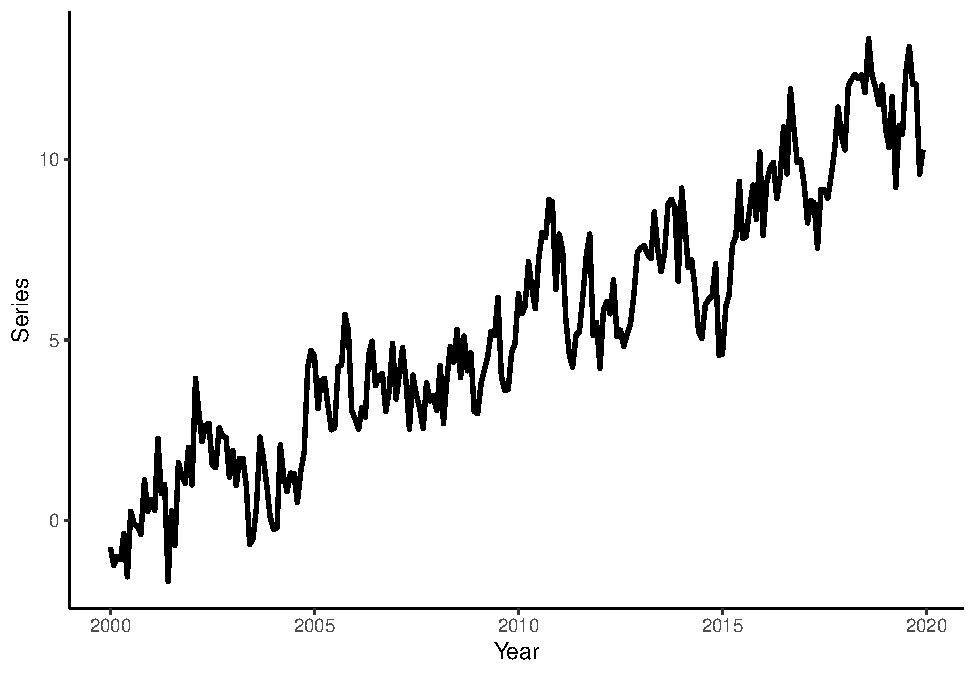
\includegraphics{forecasting_files/figure-latex/unnamed-chunk-57-1.pdf}

Calculate Akaike Information Criteria for linear, quadratic, cubic, and exponential trend models, using all observations in the series.

\begin{Shaded}
\begin{Highlighting}[]
\NormalTok{AIC\_vec }\OtherTok{\textless{}{-}} \FunctionTok{matrix}\NormalTok{(}\AttributeTok{ncol=}\DecValTok{4}\NormalTok{,}\AttributeTok{nrow=}\DecValTok{1}\NormalTok{)}
\ControlFlowTok{for}\NormalTok{(i }\ControlFlowTok{in} \DecValTok{1}\SpecialCharTok{:}\DecValTok{4}\NormalTok{)\{}
  \ControlFlowTok{if}\NormalTok{(i }\SpecialCharTok{\textless{}} \DecValTok{4}\NormalTok{)\{}
\NormalTok{    reg }\OtherTok{\textless{}{-}} \FunctionTok{lm}\NormalTok{(y}\SpecialCharTok{\textasciitilde{}}\FunctionTok{poly}\NormalTok{(trend,}\AttributeTok{degree=}\NormalTok{i,}\AttributeTok{raw=}\NormalTok{T),}\AttributeTok{data=}\NormalTok{dt)}
\NormalTok{    AIC\_vec[i] }\OtherTok{\textless{}{-}} \FunctionTok{log}\NormalTok{(}\FunctionTok{crossprod}\NormalTok{(reg}\SpecialCharTok{$}\NormalTok{residuals))}\SpecialCharTok{+}\DecValTok{2}\SpecialCharTok{*}\FunctionTok{length}\NormalTok{(reg}\SpecialCharTok{$}\NormalTok{coefficients)}\SpecialCharTok{/}\NormalTok{n}
\NormalTok{  \}}\ControlFlowTok{else}\NormalTok{\{}
\NormalTok{    reg }\OtherTok{\textless{}{-}} \FunctionTok{lm}\NormalTok{(}\FunctionTok{log}\NormalTok{(y)}\SpecialCharTok{\textasciitilde{}}\NormalTok{trend,}\AttributeTok{data=}\NormalTok{dt)}
\NormalTok{    yhat }\OtherTok{\textless{}{-}}\NormalTok{ reg}\SpecialCharTok{$}\NormalTok{fitted.values}
\NormalTok{    sig }\OtherTok{\textless{}{-}} \FunctionTok{sd}\NormalTok{(reg}\SpecialCharTok{$}\NormalTok{residuals)}
\NormalTok{    ystar }\OtherTok{\textless{}{-}} \FunctionTok{exp}\NormalTok{(yhat}\SpecialCharTok{+}\NormalTok{sig}\SpecialCharTok{\^{}}\DecValTok{2}\SpecialCharTok{/}\DecValTok{2}\NormalTok{)}
\NormalTok{    res }\OtherTok{\textless{}{-}}\NormalTok{ dt}\SpecialCharTok{$}\NormalTok{y}\SpecialCharTok{{-}}\NormalTok{ystar}
\NormalTok{    AIC\_vec[i] }\OtherTok{\textless{}{-}} \FunctionTok{log}\NormalTok{(}\FunctionTok{crossprod}\NormalTok{(res))}\SpecialCharTok{+}\DecValTok{2}\SpecialCharTok{*}\FunctionTok{length}\NormalTok{(reg}\SpecialCharTok{$}\NormalTok{coefficients)}\SpecialCharTok{/}\NormalTok{n}
\NormalTok{  \}}
\NormalTok{\}}

\NormalTok{AIC\_vec}
\end{Highlighting}
\end{Shaded}

\begin{verbatim}
##          [,1]     [,2]     [,3]     [,4]
## [1,] 8.879646 7.841645 7.849521 7.975999
\end{verbatim}

Generate a sequence of one-step-ahead forecasts from linear, quadratic, cubic, and exponential trend models, using the rolling window scheme, where the first rolling window ranges from period 1 to period 120.

\begin{Shaded}
\begin{Highlighting}[]
\NormalTok{dt}\SpecialCharTok{$}\NormalTok{t1 }\OtherTok{\textless{}{-}} \ConstantTok{NA}
\NormalTok{dt}\SpecialCharTok{$}\NormalTok{t2 }\OtherTok{\textless{}{-}} \ConstantTok{NA}
\NormalTok{dt}\SpecialCharTok{$}\NormalTok{t3 }\OtherTok{\textless{}{-}} \ConstantTok{NA}
\NormalTok{dt}\SpecialCharTok{$}\NormalTok{te }\OtherTok{\textless{}{-}} \ConstantTok{NA}

\NormalTok{R }\OtherTok{\textless{}{-}} \DecValTok{120}
\NormalTok{P }\OtherTok{\textless{}{-}}\NormalTok{ n}\SpecialCharTok{{-}}\NormalTok{R}
\ControlFlowTok{for}\NormalTok{(i }\ControlFlowTok{in} \DecValTok{1}\SpecialCharTok{:}\NormalTok{P)\{}
\NormalTok{  reg1 }\OtherTok{\textless{}{-}} \FunctionTok{lm}\NormalTok{(y}\SpecialCharTok{\textasciitilde{}}\NormalTok{trend,}\AttributeTok{data=}\NormalTok{dt[i}\SpecialCharTok{:}\NormalTok{(R}\DecValTok{{-}1}\SpecialCharTok{+}\NormalTok{i)])}
\NormalTok{  dt}\SpecialCharTok{$}\NormalTok{t1[R}\SpecialCharTok{+}\NormalTok{i] }\OtherTok{\textless{}{-}}\NormalTok{ reg1}\SpecialCharTok{$}\NormalTok{coef[}\DecValTok{1}\NormalTok{]}\SpecialCharTok{+}\NormalTok{reg1}\SpecialCharTok{$}\NormalTok{coef[}\DecValTok{2}\NormalTok{]}\SpecialCharTok{*}\NormalTok{(R}\SpecialCharTok{+}\NormalTok{i)}
  
\NormalTok{  reg2 }\OtherTok{\textless{}{-}} \FunctionTok{lm}\NormalTok{(y}\SpecialCharTok{\textasciitilde{}}\FunctionTok{poly}\NormalTok{(trend,}\AttributeTok{degree=}\DecValTok{2}\NormalTok{,}\AttributeTok{raw=}\NormalTok{T),}\AttributeTok{data=}\NormalTok{dt[i}\SpecialCharTok{:}\NormalTok{(R}\DecValTok{{-}1}\SpecialCharTok{+}\NormalTok{i)])}
\NormalTok{  dt}\SpecialCharTok{$}\NormalTok{t2[R}\SpecialCharTok{+}\NormalTok{i] }\OtherTok{\textless{}{-}}\NormalTok{ reg2}\SpecialCharTok{$}\NormalTok{coef[}\DecValTok{1}\NormalTok{]}\SpecialCharTok{+}\NormalTok{reg2}\SpecialCharTok{$}\NormalTok{coef[}\DecValTok{2}\NormalTok{]}\SpecialCharTok{*}\NormalTok{(R}\SpecialCharTok{+}\NormalTok{i)}\SpecialCharTok{+}\NormalTok{reg2}\SpecialCharTok{$}\NormalTok{coef[}\DecValTok{3}\NormalTok{]}\SpecialCharTok{*}\NormalTok{((R}\SpecialCharTok{+}\NormalTok{i)}\SpecialCharTok{\^{}}\DecValTok{2}\NormalTok{)}
  
\NormalTok{  reg3 }\OtherTok{\textless{}{-}} \FunctionTok{lm}\NormalTok{(y}\SpecialCharTok{\textasciitilde{}}\FunctionTok{poly}\NormalTok{(trend,}\AttributeTok{degree=}\DecValTok{3}\NormalTok{,}\AttributeTok{raw=}\NormalTok{T),}\AttributeTok{data=}\NormalTok{dt[i}\SpecialCharTok{:}\NormalTok{(R}\DecValTok{{-}1}\SpecialCharTok{+}\NormalTok{i)])}
\NormalTok{  dt}\SpecialCharTok{$}\NormalTok{t3[R}\SpecialCharTok{+}\NormalTok{i] }\OtherTok{\textless{}{-}}\NormalTok{ reg3}\SpecialCharTok{$}\NormalTok{coef[}\DecValTok{1}\NormalTok{]}\SpecialCharTok{+}\NormalTok{reg3}\SpecialCharTok{$}\NormalTok{coef[}\DecValTok{2}\NormalTok{]}\SpecialCharTok{*}\NormalTok{(R}\SpecialCharTok{+}\NormalTok{i)}\SpecialCharTok{+}\NormalTok{reg3}\SpecialCharTok{$}\NormalTok{coef[}\DecValTok{3}\NormalTok{]}\SpecialCharTok{*}\NormalTok{((R}\SpecialCharTok{+}\NormalTok{i)}\SpecialCharTok{\^{}}\DecValTok{2}\NormalTok{)}\SpecialCharTok{+}\NormalTok{reg3}\SpecialCharTok{$}\NormalTok{coef[}\DecValTok{4}\NormalTok{]}\SpecialCharTok{*}\NormalTok{((R}\SpecialCharTok{+}\NormalTok{i)}\SpecialCharTok{\^{}}\DecValTok{3}\NormalTok{)}
  
\NormalTok{  rege }\OtherTok{\textless{}{-}} \FunctionTok{lm}\NormalTok{(}\FunctionTok{log}\NormalTok{(y)}\SpecialCharTok{\textasciitilde{}}\NormalTok{trend,}\AttributeTok{data=}\NormalTok{dt[i}\SpecialCharTok{:}\NormalTok{(R}\DecValTok{{-}1}\SpecialCharTok{+}\NormalTok{i)])}
\NormalTok{  sig }\OtherTok{\textless{}{-}} \FunctionTok{sd}\NormalTok{(rege}\SpecialCharTok{$}\NormalTok{residuals)}
\NormalTok{  dt}\SpecialCharTok{$}\NormalTok{te[R}\SpecialCharTok{+}\NormalTok{i] }\OtherTok{\textless{}{-}} \FunctionTok{exp}\NormalTok{(rege}\SpecialCharTok{$}\NormalTok{coef[}\DecValTok{1}\NormalTok{]}\SpecialCharTok{+}\NormalTok{rege}\SpecialCharTok{$}\NormalTok{coef[}\DecValTok{2}\NormalTok{]}\SpecialCharTok{*}\NormalTok{(R}\SpecialCharTok{+}\NormalTok{i)}\SpecialCharTok{+}\NormalTok{sig}\SpecialCharTok{\^{}}\DecValTok{2}\SpecialCharTok{/}\DecValTok{2}\NormalTok{)}
\NormalTok{\}}
\end{Highlighting}
\end{Shaded}

Plot the original series overlay by the one-step-ahead forecasts from the four considered trend models. Note, for convenience we will first `melt' the data.table in to the `long' format.

\begin{Shaded}
\begin{Highlighting}[]
\NormalTok{dt\_long }\OtherTok{\textless{}{-}} \FunctionTok{melt}\NormalTok{(dt[,.(date,y,}\AttributeTok{linear=}\NormalTok{t1,}\AttributeTok{quadratic=}\NormalTok{t2,}\AttributeTok{cubic=}\NormalTok{t3,}\AttributeTok{exponential=}\NormalTok{te)],}\AttributeTok{id.vars=}\StringTok{"date"}\NormalTok{)}

\FunctionTok{ggplot}\NormalTok{(dt\_long,}\FunctionTok{aes}\NormalTok{(}\AttributeTok{x=}\NormalTok{date,}\AttributeTok{y=}\NormalTok{value,}\AttributeTok{color=}\NormalTok{variable))}\SpecialCharTok{+}
  \FunctionTok{geom\_line}\NormalTok{(}\AttributeTok{size=}\DecValTok{1}\NormalTok{,}\AttributeTok{na.rm=}\NormalTok{T)}\SpecialCharTok{+}
  \FunctionTok{scale\_color\_manual}\NormalTok{(}\AttributeTok{values=}\FunctionTok{c}\NormalTok{(}\StringTok{"darkgray"}\NormalTok{,}\StringTok{"black"}\NormalTok{,}\StringTok{"goldenrod"}\NormalTok{,}\StringTok{"steelblue"}\NormalTok{,}\StringTok{"indianred"}\NormalTok{))}\SpecialCharTok{+}
  \FunctionTok{labs}\NormalTok{(}\AttributeTok{x=}\StringTok{"Year"}\NormalTok{,}\AttributeTok{y=}\StringTok{"Trending Series and Forecasts"}\NormalTok{)}\SpecialCharTok{+}
  \FunctionTok{theme\_classic}\NormalTok{()}\SpecialCharTok{+}
  \FunctionTok{theme}\NormalTok{(}\AttributeTok{legend.title=}\FunctionTok{element\_blank}\NormalTok{(),}\AttributeTok{legend.position=}\FunctionTok{c}\NormalTok{(.}\DecValTok{15}\NormalTok{,.}\DecValTok{85}\NormalTok{))}
\end{Highlighting}
\end{Shaded}

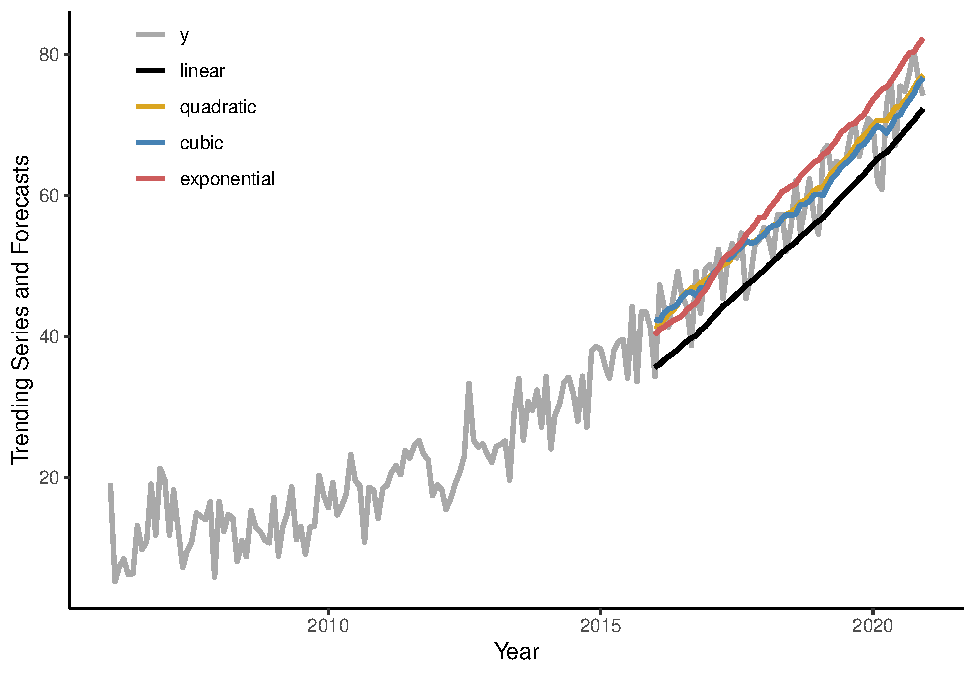
\includegraphics{forecasting_files/figure-latex/unnamed-chunk-60-1.pdf}

Calculate the RMSFE measures for each of the two forecasting methods.

\begin{Shaded}
\begin{Highlighting}[]
\NormalTok{dt[,}\StringTok{\textasciigrave{}}\AttributeTok{:=}\StringTok{\textasciigrave{}}\NormalTok{(}\AttributeTok{e\_t1=}\NormalTok{y}\SpecialCharTok{{-}}\NormalTok{t1,}\AttributeTok{e\_t2=}\NormalTok{y}\SpecialCharTok{{-}}\NormalTok{t2,}\AttributeTok{e\_t3=}\NormalTok{y}\SpecialCharTok{{-}}\NormalTok{t3,}\AttributeTok{e\_te=}\NormalTok{y}\SpecialCharTok{{-}}\NormalTok{te)]}

\NormalTok{rmsfe\_t1 }\OtherTok{\textless{}{-}} \FunctionTok{sqrt}\NormalTok{(}\FunctionTok{mean}\NormalTok{(dt}\SpecialCharTok{$}\NormalTok{e\_t1}\SpecialCharTok{\^{}}\DecValTok{2}\NormalTok{,}\AttributeTok{na.rm=}\NormalTok{T))}
\NormalTok{rmsfe\_t2 }\OtherTok{\textless{}{-}} \FunctionTok{sqrt}\NormalTok{(}\FunctionTok{mean}\NormalTok{(dt}\SpecialCharTok{$}\NormalTok{e\_t2}\SpecialCharTok{\^{}}\DecValTok{2}\NormalTok{,}\AttributeTok{na.rm=}\NormalTok{T))}
\NormalTok{rmsfe\_t3 }\OtherTok{\textless{}{-}} \FunctionTok{sqrt}\NormalTok{(}\FunctionTok{mean}\NormalTok{(dt}\SpecialCharTok{$}\NormalTok{e\_t3}\SpecialCharTok{\^{}}\DecValTok{2}\NormalTok{,}\AttributeTok{na.rm=}\NormalTok{T))}
\NormalTok{rmsfe\_te }\OtherTok{\textless{}{-}} \FunctionTok{sqrt}\NormalTok{(}\FunctionTok{mean}\NormalTok{(dt}\SpecialCharTok{$}\NormalTok{e\_te}\SpecialCharTok{\^{}}\DecValTok{2}\NormalTok{,}\AttributeTok{na.rm=}\NormalTok{T))}

\NormalTok{rmsfe\_t1}
\end{Highlighting}
\end{Shaded}

\begin{verbatim}
## [1] 6.151904
\end{verbatim}

\begin{Shaded}
\begin{Highlighting}[]
\NormalTok{rmsfe\_t2}
\end{Highlighting}
\end{Shaded}

\begin{verbatim}
## [1] 3.796861
\end{verbatim}

\begin{Shaded}
\begin{Highlighting}[]
\NormalTok{rmsfe\_t3}
\end{Highlighting}
\end{Shaded}

\begin{verbatim}
## [1] 3.906023
\end{verbatim}

\begin{Shaded}
\begin{Highlighting}[]
\NormalTok{rmsfe\_te}
\end{Highlighting}
\end{Shaded}

\begin{verbatim}
## [1] 5.132312
\end{verbatim}

\end{document}
